\documentclass{beamer}

\usepackage{amsmath}
\usepackage{amssymb}
\usepackage{booktabs}
\usepackage{rotating}
\usepackage{multirow}
\usepackage{colortbl,color}
\usepackage{graphics}

\usepackage{colortbl,color}
\usetheme{material}
\useLightTheme
\usePrimaryRed
\useAccentGreen

\renewcommand{\theenumii}{\alph{\enumii}}
\defbeamertemplate{itemize subitem}{dash}{--}
\defbeamertemplate{itemize subsubitem}{dash}{--}
\setbeamertemplate{itemize item}[circle]
\setbeamertemplate{itemize subitem}[dash]
\setbeamertemplate{itemize subsubitem}[dash]
\setbeamertemplate{enumerate item}{\arabic{enumi}.}
\setbeamertemplate{enumerate subitem}{(\alph{enumii})}
\usefoottemplate{}

\setbeamertemplate{headline}{}
\usenavigationsymbolstemplate{}


\newcommand{\SD}[1]{{\tiny $\left(#1\right)$}}
\newcommand{\SDm}[1]{{\tiny \left(#1\right)}}
\newcommand{\Prob}[1]{\mbox{Pr}\left\{#1\right\}}
\newcommand{\CProb}[2]{\mbox{Pr}\left\{#1\left|#2\right.\right\}}

\usepackage{array}
\newcolumntype{P}[1]{>{\centering\arraybackslash}p{#1}}

\begin{document}
\section{Intro}
\title{\LARGE Econ 2220: Experimental Economics \\ Communication 2}
\author{Alistair J. Wilson }
\date{Fall 2020}
 \maketitle

\begin{frame}{Communication Intro}
	\begin{card}
	Communication:
		\begin{enumerate}
			\item Coordination
			\item \textbf{Information Transmission}
			\item Analogy \& Instruction
		\end{enumerate}
	\end{card}
\end{frame}
\section{Intro}
\begin{frame}
	\begin{card}[Information Transmission timing]
			\begin{enumerate}
				\item One player has information on a state of the world $\theta\in\Theta$
				\item \textbf{Sends} a message $m$ to an uninformed player
				\item Uninformed player \textbf{receives} the message and makes a choice $x\in X$ 
			\end{enumerate}
\end{card}
\pause
\begin{card}	
		General preferences are given by $u_S(\theta,m,x)$ and $v_R(\theta,m,x)$
	\end{card}
\end{frame}

\begin{frame}
	\begin{card}[Solution Concepts]
Main concept is Bayesian Nash Equilibrium, but might also look at refinements:
		\begin{itemize}
			\item Sequential Equilibrium
			\item Perfect Equilibrium
			\item Intuitive Criterion
			\item Divinity \& D1 etc.
			\item Stability
		\end{itemize}
\end{card}
		\pause
\begin{card}
See Kreps\&Wilson EMA 82, Cho\&Kreps QJE 87, Kohlberg\&Mertens EMA 86, etc. for theory

See Banks, Camerer \& Porter (GEB 96) for experiment on these refinements
\end{card}
\end{frame}

\begin{frame}
	\begin{card}[Cheap Talk Restrictions]
			\begin{itemize}
				\item $u(\theta,m,x)=u(\theta,m^\prime,x)$ and $v(\theta,m,x)=v(\theta,m^\prime,x)$
				$\forall m,m^\prime\in M$ 
				\item $M(\theta)=M,\forall\theta\in\Theta$
				\item $X(\theta,m)=X,\forall\theta\in\Theta,\forall m\in M$
			\end{itemize}
\end{card}
			\pause
\begin{card}
Messages under cheap talk:
			\begin{itemize}
				\item do not directly affect payoffs
				\item do not restrict the action set
				\item are available for all states
			\end{itemize}
\end{card}
\end{frame}

\section{Crawford \& Sobel (EMA 1982)}

\begin{frame}
\begin{card}[Crawford \& Sobel 1982 Setup]
	\begin{itemize}
		\item State $\theta$ drawn on interval $\Theta$ according to some distribution
		\item Receiver preferences over action $x\in X=\Theta$ are $$v^R(x,\theta)=-\left\|x-\theta \right\|$$
		\item Sender preferences are $$u^S(x,\theta)=-\left\|x+b-\theta \right\|$$
		where $b$ is the preference misalignment
	\end{itemize}
\end{card}
\end{frame}

\begin{frame}
\begin{card}[Crawford \& Sobel 1982 Timing]
		\begin{enumerate}[i)]
		\item State $\theta$ drawn, Sender observes
		\item Sender chooses message $m\in M$
		\item Receiver observes $m$, choose action $x$
		\end{enumerate}
\end{card}
\end{frame}

\begin{frame}{Crawford-Sobel Example}
	\begin{center}
		\includegraphics<1>[width=1.0\textwidth]{./i/CSexample-1.eps}
		\includegraphics<2>[width=1.0\textwidth]{./i/CSexample-2.eps}
		\includegraphics<3-5>[width=1.0\textwidth]{./i/CSexample-3.eps}
		\includegraphics<6>[width=1.0\textwidth]{./i/CSexample-9.eps}
		\includegraphics<7>[width=1.0\textwidth]{./i/CSexample-10.eps}
		\includegraphics<8>[width=1.0\textwidth]{./i/CSexample-11.eps}
		\includegraphics<9>[width=1.0\textwidth]{./i/CSexample-12.eps}
		\includegraphics<10>[width=1.0\textwidth]{./i/CSexample-13.eps}
		\includegraphics<11>[width=1.0\textwidth]{./i/CSexample-14.eps}
	\end{center}
	
	\only<1-2>{State realized}
	\only<3>{Sender has optimal point $b$ to right of $\theta$}
	\only<4>{Sender sends a message $m(\theta)$}
	\only<5>{Receiver makes a choice $x(m)$, optimal point of $\theta$}
	\only<6>{Sender could reveal truth with $m(\theta)=\theta$.}
	\only<7>{In which case the Receiver chooses their best point}
	\only<8>{Not an equilibrium, as now the sender exaggerates...}
	\only<9>{...to which the receiver reacts...}
	\only<10>{...and on...}
	\only<11>{...and on.}
\end{frame}

\begin{frame}{Crawford-Sobel Equilibrium}
	\begin{center}
		\includegraphics<1>[width=1.0\textwidth]{./i/CSexample-Eq1.eps}
		\includegraphics<2>[width=1.0\textwidth]{./i/CSexample-Eq1b.eps}
		\includegraphics<3>[width=1.0\textwidth]{./i/CSexample-Eq2.eps}
		\includegraphics<4>[width=1.0\textwidth]{./i/CSexample-Eq2b.eps}
		\includegraphics<5>[width=1.0\textwidth]{./i/CSexample-Eq3.eps}
		\includegraphics<6-8>[width=1.0\textwidth]{./i/CSexample-Eq3b.eps}
	\end{center}
	
	\only<1-2>{Babbling, meaningless message}
	\only<3-4>{Partial Revelation, like ``Low'' or ``High''}
	\only<5-6>{Partial Revelation, Like ``Low'', ``Medium'' or ``High''}
	\only<7>{More messages are more informative}
	\only<8>{Message identities are meaningless}
\end{frame}

\section{Dickhaut, McCabe Mukherji (ET 1994)}
\begin{frame}{Dickhaut, McCabe Mukherji (ET 1994)}
\begin{card}
	\begin{itemize}
		\item Four possible states $\Theta=\left\{1,2,3,4 \right\}$
		\item Four possible actions $X=\left\{1,2,3,4 \right\}$
		\item Preferences of the receiver are:
				$$v^R(x,\theta)=C_R-a\cdot \left|x-\theta\right|^{1.1}$$
				and for the sender are:
				$$u^S(x,\theta;b)=C_S-a\cdot \left|x-\theta-b\right|^{1.1}$$
		\item Treatment variable is $-b$, which takes on values in $\left\{0.25,0.5,1.0,2.0,3.0\right\}$
	\end{itemize}
	\end{card}
\end{frame}

\begin{frame}
\begin{card}[Treatment]
$b=0.25$:

    \begin{center}
	    \begin{tabular}{r|c|c|c|c|} 
			\multicolumn{1}{r}{ }& \multicolumn{4}{c}{State:}		\\
			\multicolumn{1}{r}{ }& \multicolumn{1}{c}{$\theta=1$}  & \multicolumn{1}{c}{$\theta=2$} & \multicolumn{1}{c}{$\theta=3$}& \multicolumn{1}{c}{$\theta=4$} \\ \cline{2-5}
			$x=1$ &  $206,274$ & $176,214$  & $108,145$ & $37,73$  \\ \cline{2-5}
			$x=2$ &  $143,214$ & $206,274$  & $176,214$ & $108,145$ \\ \cline{2-5}
			$x=3$ &  $73,145$  & $143,214$  & $206,274$ & $176,214$  \\ \cline{2-5}
			$x=4$ &  $0,73$    & $73,145$   & $143,214$ & $206,274$    \\ \cline{2-5}
		\end{tabular}
	\end{center}
\end{card}
\end{frame}

\begin{frame}
\begin{card}[Treatment]
$b=0.5$:

\begin{center}
	\begin{tabular}{r|c|c|c|c|} 
			\multicolumn{1}{r}{ }& \multicolumn{4}{c}{State:}		\\
			\multicolumn{1}{r}{ }& \multicolumn{1}{c}{$\theta=1$}  & \multicolumn{1}{c}{$\theta=2$} & \multicolumn{1}{c}{$\theta=3$}& \multicolumn{1}{c}{$\theta=4$} \\ \cline{2-5}
			$x=1$ &  $242,274$ & $242,214$  & $176,145$ & $105,73$  \\ \cline{2-5}
			$x=2$ &  $176,214$ & $242,274$  & $242,214$ & $176,145$ \\ \cline{2-5}
			$x=3$ &  $105,145$ & $176,214$  & $242,274$ & $242,214$  \\ \cline{2-5}
			$x=4$ &  $31,73$   & $105,145$  & $176,214$ & $242,274$    \\ \cline{2-5}
		\end{tabular}
	\end{center}
\end{card}
\end{frame}

\begin{frame}
\begin{card}[Treatment]
$b=1$:

\begin{center}
	\begin{tabular}{r|c|c|c|c|} 
			\multicolumn{1}{r}{ }& \multicolumn{4}{c}{State:}		\\
			\multicolumn{1}{r}{ }& \multicolumn{1}{c}{$\theta=1$}  & \multicolumn{1}{c}{$\theta=2$} & \multicolumn{1}{c}{$\theta=3$}& \multicolumn{1}{c}{$\theta=4$} \\ \cline{2-5}
			$x=1$ &  $216,274$ & $276,214$  & $216,145$ & $147,73$  \\ \cline{2-5}
			$x=2$ &  $147,214$ & $216,274$  & $276,214$ & $216,145$ \\ \cline{2-5}
			$x=3$ &  $75,145$  & $147,214$  & $216,274$ & $276,214$  \\ \cline{2-5}
			$x=4$ &  $0,73$    & $75,145$   & $147,214$ & $216,274$    \\ \cline{2-5}
		\end{tabular}
	\end{center}
\end{card}
\end{frame}

\begin{frame}{Dickhaut, McCabe Mukherji (ET 1994)}
\begin{card}[Treatment]
$b=2$:
\begin{center}
	\begin{tabular}{r|c|c|c|c|} 
			\multicolumn{1}{r}{ }& \multicolumn{4}{c}{State:}		\\
			\multicolumn{1}{r}{ }& \multicolumn{1}{c}{$\theta=1$}  & \multicolumn{1}{c}{$\theta=2$} & \multicolumn{1}{c}{$\theta=3$}& \multicolumn{1}{c}{$\theta=4$} \\ \cline{2-5}
			$x=1$ &  $224,274$ & $293,214$  & $353,145$ & $293,73$  \\ \cline{2-5}
			$x=2$ &  $152,214$ & $224,274$  & $293,214$ & $353,145$ \\ \cline{2-5}
			$x=3$ &  $77,145$  & $152,214$  & $224,274$ & $293,214$  \\ \cline{2-5}
			$x=4$ &  $0,73$    & $77,145$   & $152,214$ & $224,274$    \\ \cline{2-5}
		\end{tabular}
	\end{center}
\end{card}
\end{frame}

\begin{frame}{Dickhaut, McCabe Mukherji (ET 1994)}
    \begin{card}[Treatment]
$b=3$:
    \begin{center}
    	\begin{tabular}{r|c|c|c|c|} 
    			\multicolumn{1}{r}{ }& \multicolumn{4}{c}{State:}		\\
    			\multicolumn{1}{r}{ }& \multicolumn{1}{c}{$\theta=1$}  & \multicolumn{1}{c}{$\theta=2$} & \multicolumn{1}{c}{$\theta=3$}& \multicolumn{1}{c}{$\theta=4$} \\ \cline{2-5}
    			$x=1$ &  $230,274$ & $302,214$  & $371,145$ & $431,73$  \\ \cline{2-5}
    			$x=2$ &  $155,214$ & $230,274$  & $302,214$ & $371,145$ \\ \cline{2-5}
    			$x=3$ &  $78,145$  & $155,214$  & $230,274$ & $302,214$  \\ \cline{2-5}
    			$x=4$ &  $0,73$    & $78,145$   & $155,214$  & $230,274$    \\ \cline{2-5}
    		\end{tabular}
    	\end{center}
    \end{card}
\end{frame}

\begin{frame}{Dickhaut, McCabe Mukherji (ET 1994)}
    \begin{card}
    The message space is the union of:
    	\begin{itemize}
    		\item $\left\{ 1\right\}$,$\left\{ 2\right\}$,$\left\{ 3\right\}$,$\left\{ 4\right\}$
    		\item $\left\{ 1,2\right\}$,$\left\{ 2,3\right\}$,$\left\{ 3,4\right\}$
    		\item $\left\{ 1,2,3\right\}$,$\left\{ 2,3,4\right\}$
    		\item $\left\{ 1,2,3,4\right\}$
    	\end{itemize}
    \end{card}
\end{frame}

\begin{frame}{Dickhaut, McCabe Mukherji (ET 1994)}
\begin{card}
    \begin{itemize}
    	\item All of the games have a babbling equilibrium
    	\item Focus on truthful-language equilibria
    	\item Games with $b=0.25$ and $b=0.5$ have a truth-telling equilibrium, as well as other
    	\item Game with $b=1.0$ has two meaningful equilibria, welfare ranked
    	\item Games with $b=2.0$ and $b=3.0$ have only babbling equilibria
    \end{itemize}
\end{card}
\end{frame}

\begin{frame}
\begin{card}[Experimental Details]
    \begin{itemize}
    	\item Minnesota undergrads
    	\item Nine subjects per session
    	\begin{itemize}
    		\item 4 Senders
    		\item 4 Receivers
    		\item 1 monitor: fixed \$20 payment
    	\end{itemize}
    	\item 12 periods
    	\item Between subject design, 3 sessions each treatment
    \end{itemize}
\end{card}
\end{frame}

\begin{frame}
    \begin{card}[Experimental Round Timing]
    	\begin{enumerate}
    		\item Monitor rolls a die
    		\item Informs the senders
    		\item Senders circle a message on form
    		\item Form is passed to matched receiver (pre-randomized match)
    		\item Receiver chooses action
    	\end{enumerate}
	\end{card}
\end{frame}

\begin{frame}{Dickhaut, McCabe Mukherji (ET 1994)}
\begin{card}
Look at average distance from state, $\left|\theta_{it}-x_{it}\right|$

	\begin{center}
		\begin{tabular}{lc}\hline
		Treatment &  Mean Distance \\\hline
		 $b=0.25$ &  0.36 \\ 
		 $b=0.5$  &  0.35 \\
		 $b=1.0$  &  0.56 \\
		 $b=2.0$  &  0.72 \\
		 $b=3.0$  &  0.92 \\\hline
		 \end{tabular}
	 \end{center}
	\end{card}
\end{frame}

\begin{frame}{Dickhaut, McCabe Mukherji (ET 1994)}

\begin{card}
\begin{itemize}
	\item Rest of the analysis is fairly confused/confusing
	\item Main takeaways are:
	\begin{itemize}
		\item Each game isn't at the Bayesian Nash equilibrium
		\item As $b$ increases less information is transmitted
		\item Coarser information types are consistent
	\end{itemize}
\end{itemize}
\end{card}
\end{frame}

\section{Cai \& Wang (GEB 2006)}
\begin{frame}{Cai \& Wang (GEB 2006)}
\begin{card}
	\begin{itemize}
		\item Similar motivation to Dickhaut, McCabe and Mukherji (1994)
		\item More bells, more whistles:
		\begin{itemize}
			\item Better data analysis
			\item Two behavioral explanatory models
			\item Document overcommunication
		\end{itemize}
	\end{itemize}
\end{card}
\end{frame}

\begin{frame}{Cai \& Wang (GEB 2006)}
\begin{card}
	\begin{itemize}
		\item State space is $\Theta=\left\{1,3,5,7,9 \right\}$
		\item Preferences of the receiver are:
				$$u^R(x,\theta)=C_R-a\cdot \left|x-\theta\right|^{k}$$
				and for the sender are:
				$$v^S(x,\theta;d)=C_S-a\cdot \left|x+d-\theta\right|^{k}$$
		\item Treatments are 
		\begin{itemize}
			\item $d\in\left\{0.5,1.2,2,4 \right\}$
			\item $k=1.4$ (Robustness checks $k=1.2$, $k=1$)
		\end{itemize}
		\item Message space is $M=\Theta$ with randomization
		\item Choice space is $X=\left\{1,2,3,4,5,6,7,8,9 \right\}$
	\end{itemize}
	\end{card}
\end{frame}
\begin{frame}{Cai \& Wang (GEB 2006)}
	\begin{card}
    Theoretical predictions (most informative eqbm):
		\begin{itemize}
			\item $d=0.5\Longrightarrow$ full revelation
			\item $d=1.2\Longrightarrow x(1)=x(3)=2$, $x(5)=x(7)=x(9)=7$
			\item $d=2.0 \Longrightarrow x(1)=1, x(3)=x(5)=x(7)=x(9)=5$
			\item $d=4.0 \Longrightarrow$ Babbling equilibrium
		\end{itemize}
	\end{card}
\end{frame}
\begin{frame}
\begin{card}[Experimental Details]
	\begin{itemize}
		\item UCLA undergrads
		\item \$5 show-up
		\item Session average incentivized payment \$10.30--32.11
		\item z-Tree interface (mouselab type features)
		\item Role rotation (random)
	\end{itemize}
\end{card}
\end{frame}

\begin{frame}{Cai \& Wang (GEB 2006)}
\begin{card}
\centering 
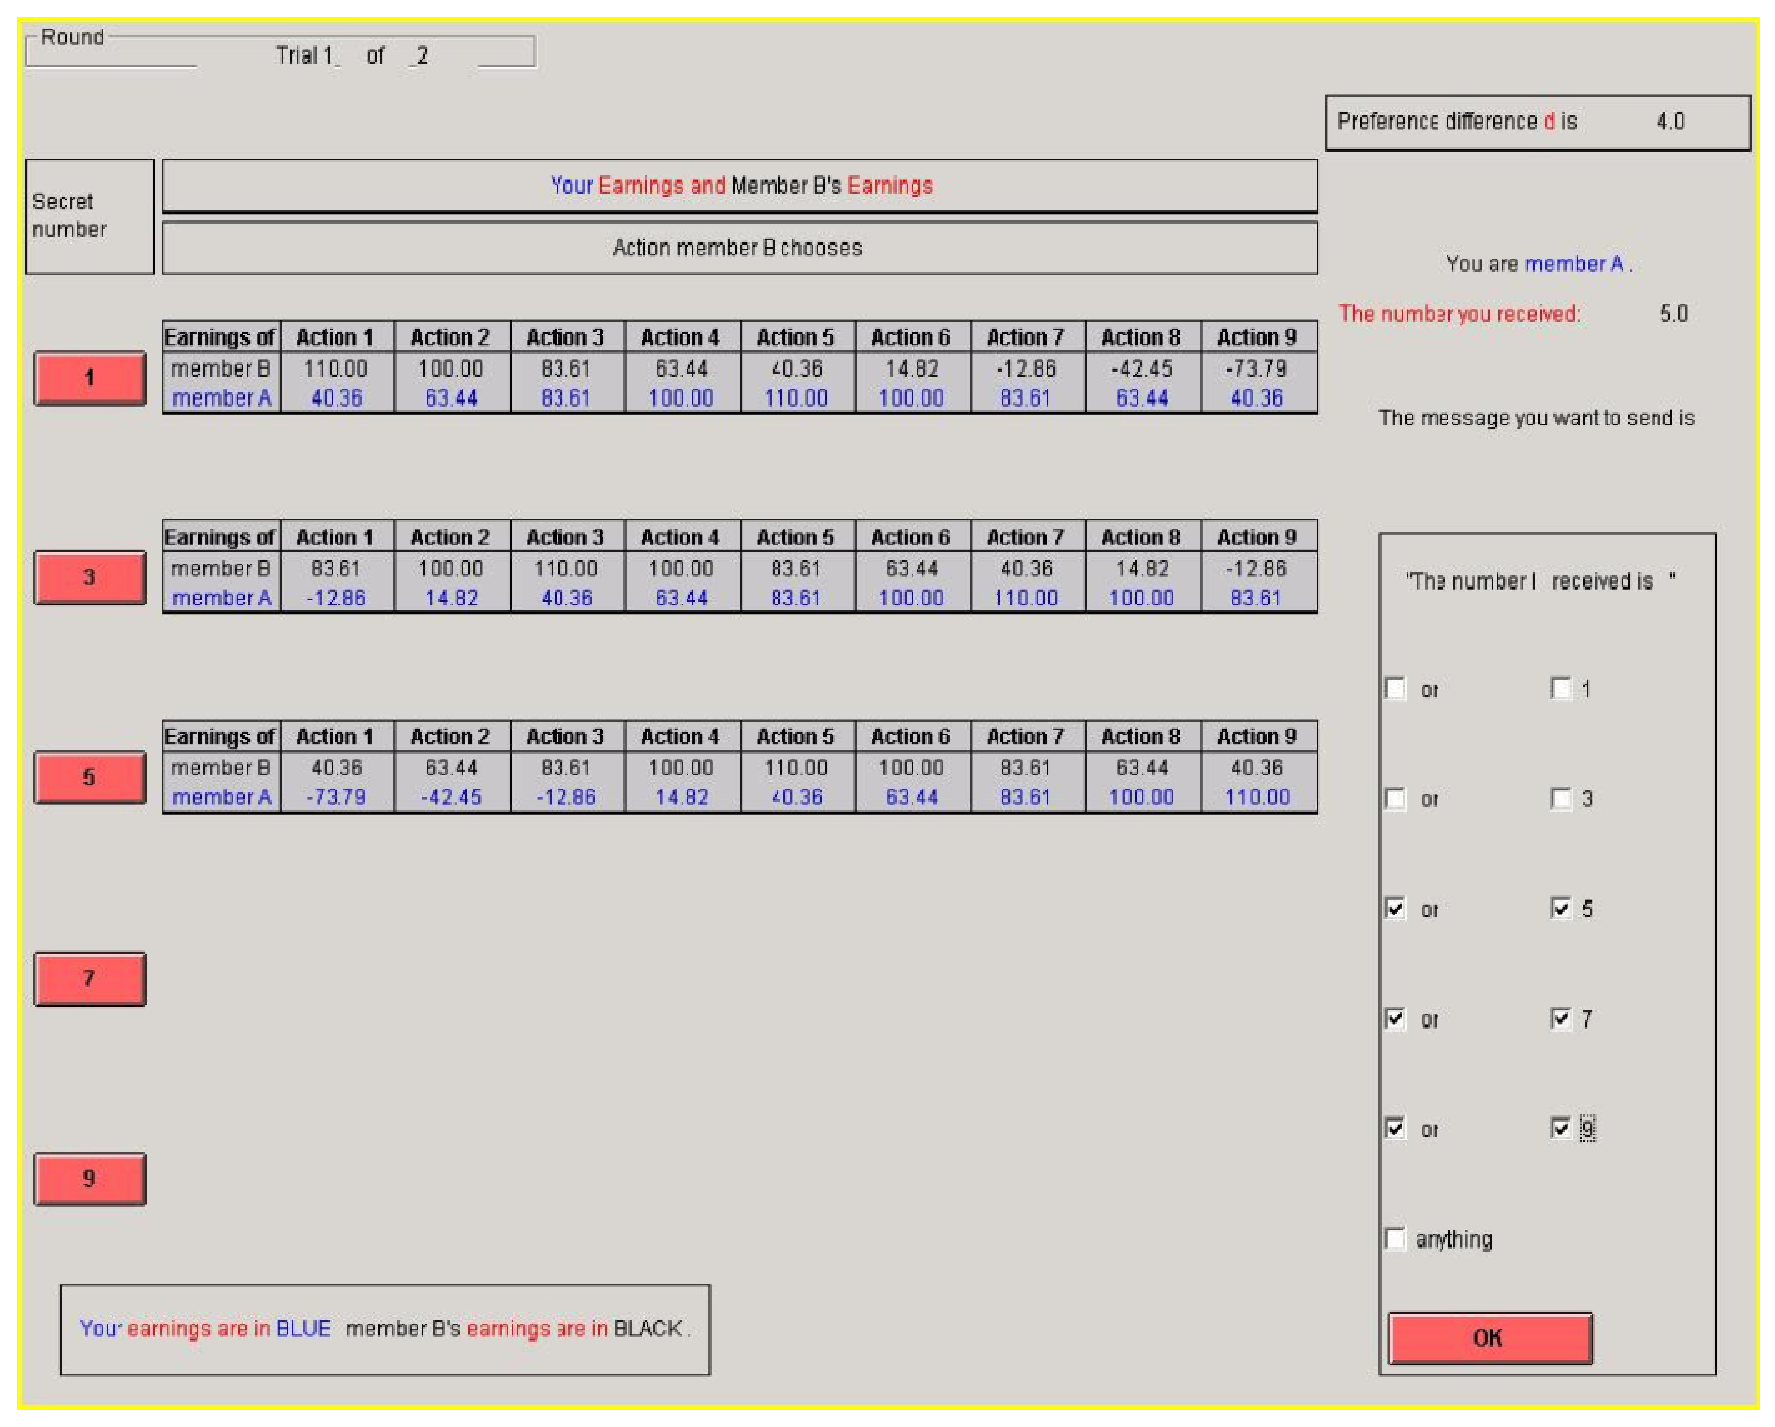
\includegraphics[height=0.65\textheight]{./i/cw2004fig1.eps}
\end{card}
\end{frame}

\begin{frame}{Cai \& Wang (GEB 2006)}
\begin{card}
\centering 
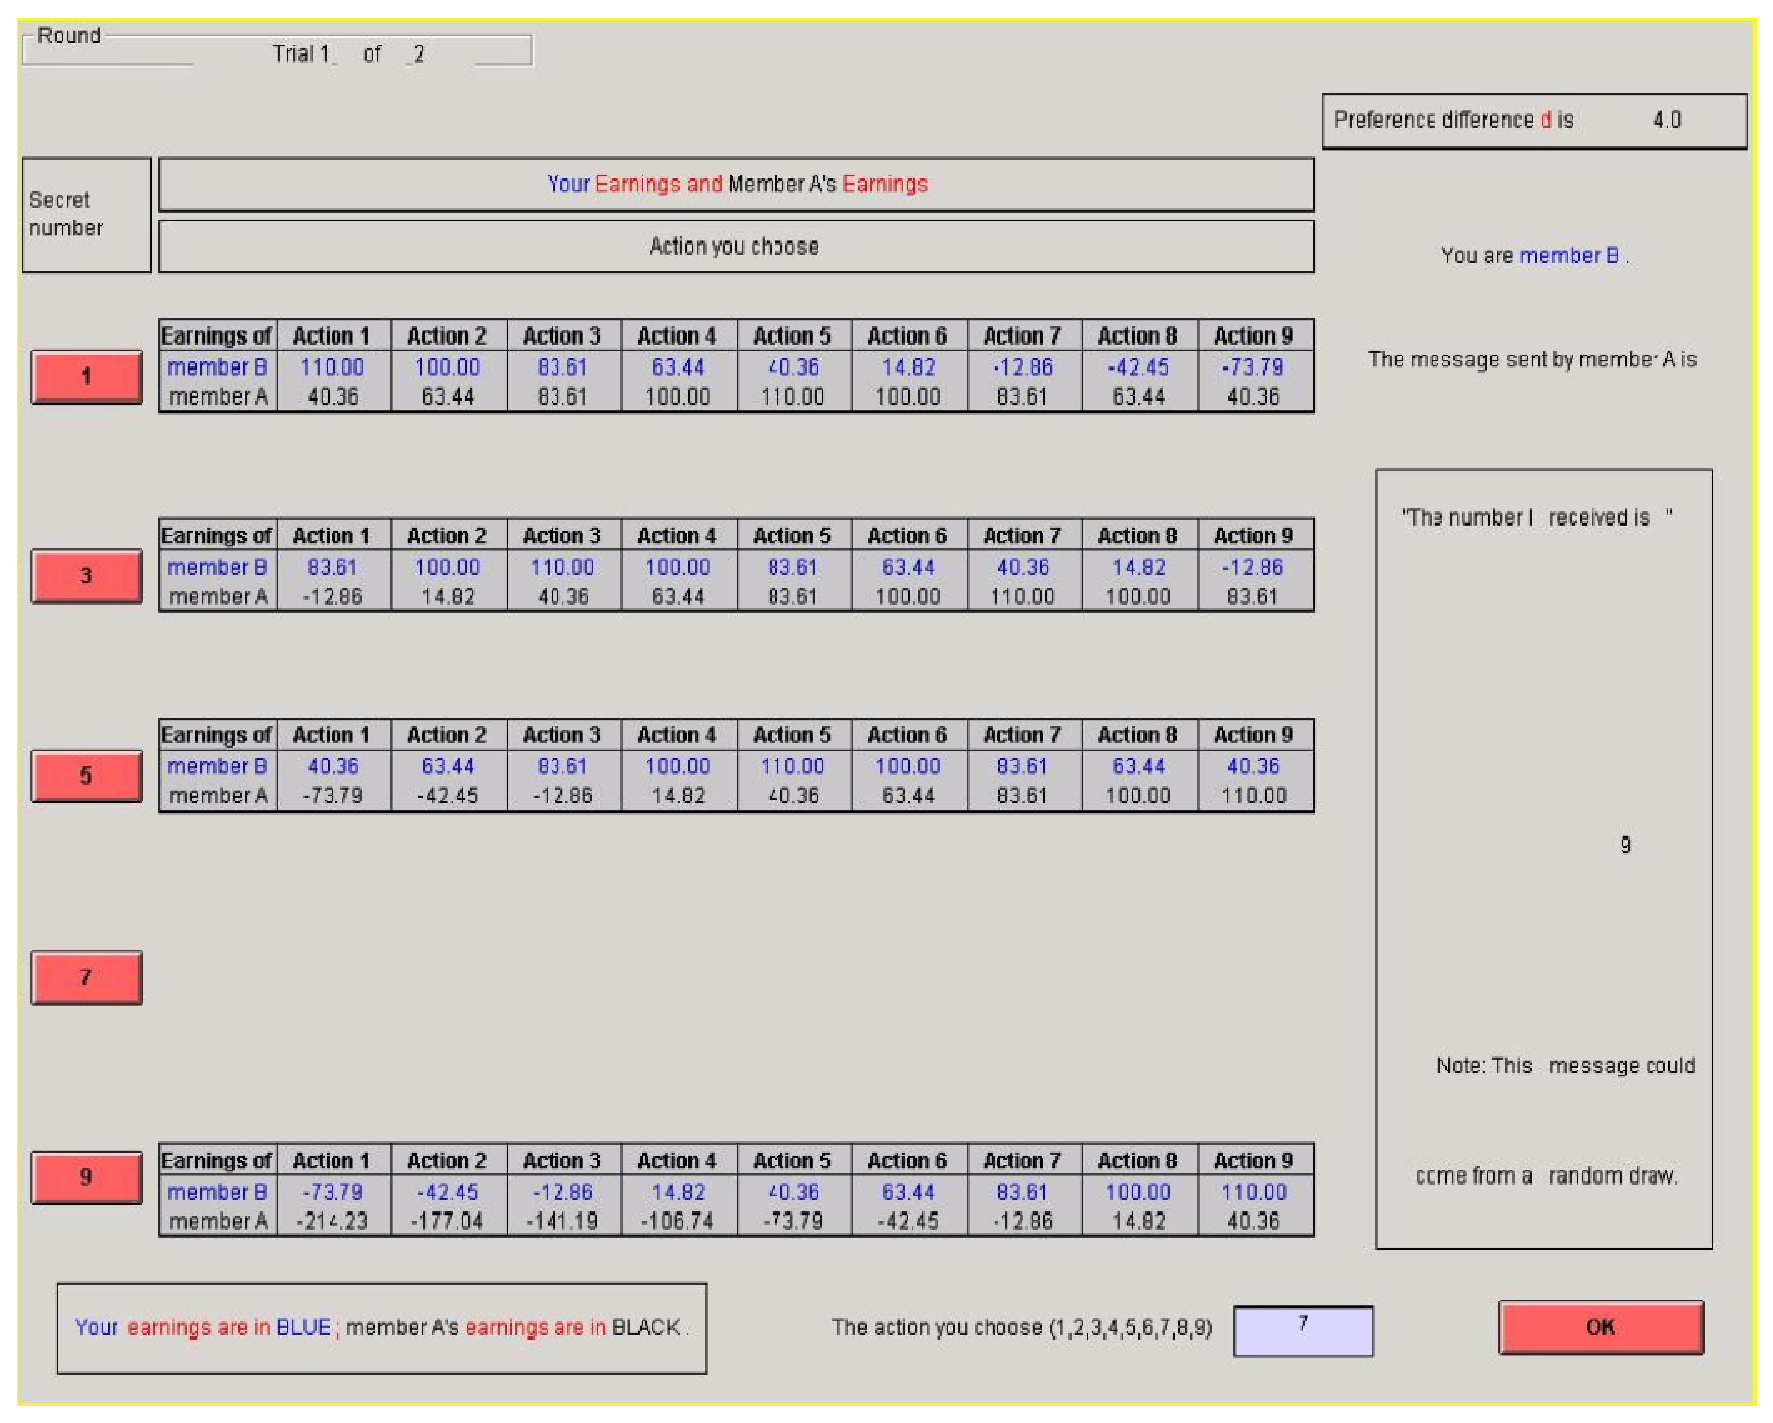
\includegraphics[height=0.65\textheight]{./i/cw2004fig2.eps}
\end{card}
\end{frame}

\begin{frame}{Cai \& Wang (GEB 2006)}
	\begin{card}
Slightly weird design:
		\begin{itemize}
			\item Subjects able to send random messages
			\item Possible loses in $d=4$ rounds
		\end{itemize}
\end{card}		
\pause
\begin{card}
Treatments are fairly ad hoc:
		\begin{itemize}
			\item 1 within-subject session (21 rounds, 28 subjects)
			\item 1 session with $d=4$ (31 rounds, 32 subjects)
			\item 1 session with $d=2$ (20 rounds, 32 subjects)
			\item 1 within session at $k=1.2$, no msg randomization
			\item 1 within session at $k=1.0$, noisy messages
		\end{itemize}
	\end{card}
\end{frame}

\begin{frame}{Cai \& Wang (GEB 2006)}
\begin{card}
\begin{center}
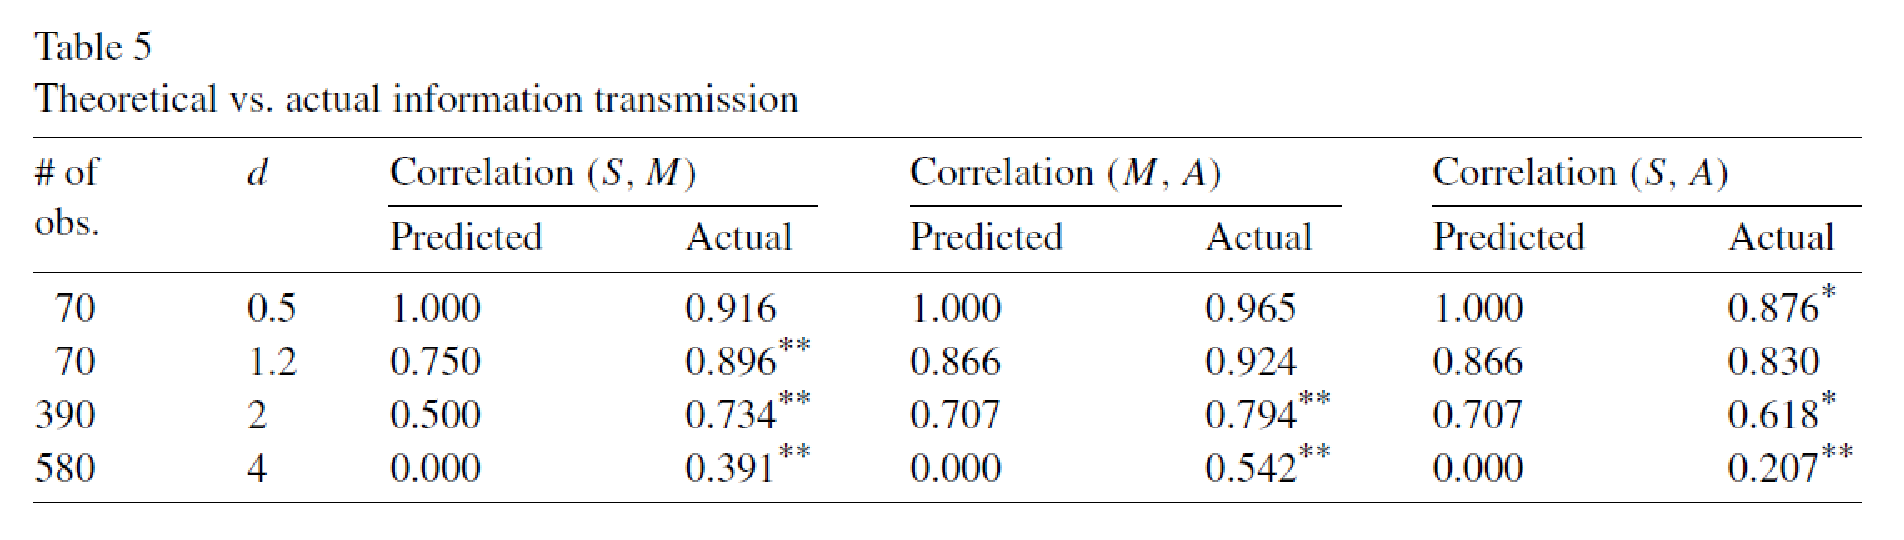
\includegraphics[width=1\textwidth]{./i/cw2006Tbl5.eps}
\end{center}
\end{card}
\begin{card}
	\begin{itemize}
		\item Comparative statics are in the theoretical direction
		\item But there is greater correlation than predicted in non-perfect alignment games
		\item Implies more truth-telling than optimal
	\end{itemize}
\end{card}
\end{frame}

\begin{frame}{Cai \& Wang (GEB 2006)}
	\begin{card}
In order to explain the data the authors fit two explanatory behavioral models
		\begin{enumerate}
			\item Quantal-Response Equilibrium

			(McKelvey \& Palfrey EE 1995, GEB 1998)
			\item Level-$k$ model (baseline honesty)
			
			(Nagel AER 1995; Stahl \& Wilson GEB 1995; Costa-Gomes et al EMA 2001; Crawford AER 2003)
		\end{enumerate}
	\end{card}
\end{frame}


\begin{frame}
	\begin{card}[ Level-$k$ model]
		\begin{enumerate}
			\setcounter{enumi}{-1}
			\item Sender honest $m_0=\theta$; Receiver Honest $x_0=m$
			\item $m_1=\theta+d ; x_1=m-d$
			\item $m_2=\theta+2 d ; x_1=m-2 d$ 
			$$\vdots$$ 
			\item[k.]  $m_k=\theta+2 k ; x_k=m-k d$
		\end{enumerate}
		\end{card}

\end{frame}

\begin{frame}{Cai \& Wang (GEB 2006)}
\begin{card}
\begin{center}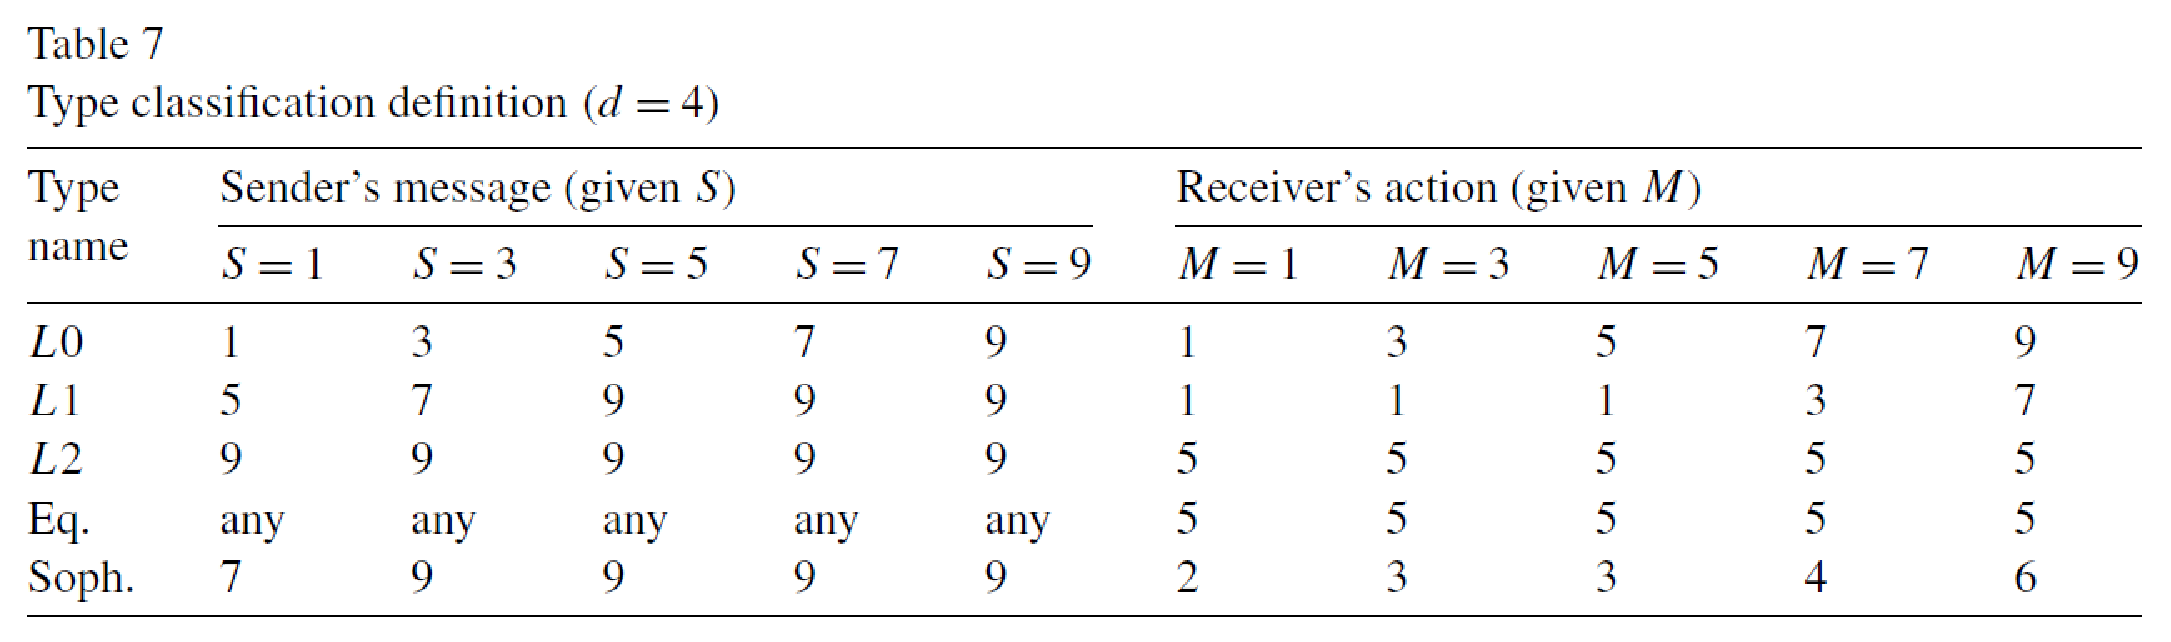
\includegraphics[width=0.98\textwidth]{./i/cw2006Tbl7.eps}\end{center}
\end{card}
\end{frame}
\begin{frame}{Cai \& Wang (GEB 2006)}
\begin{card}
\begin{center}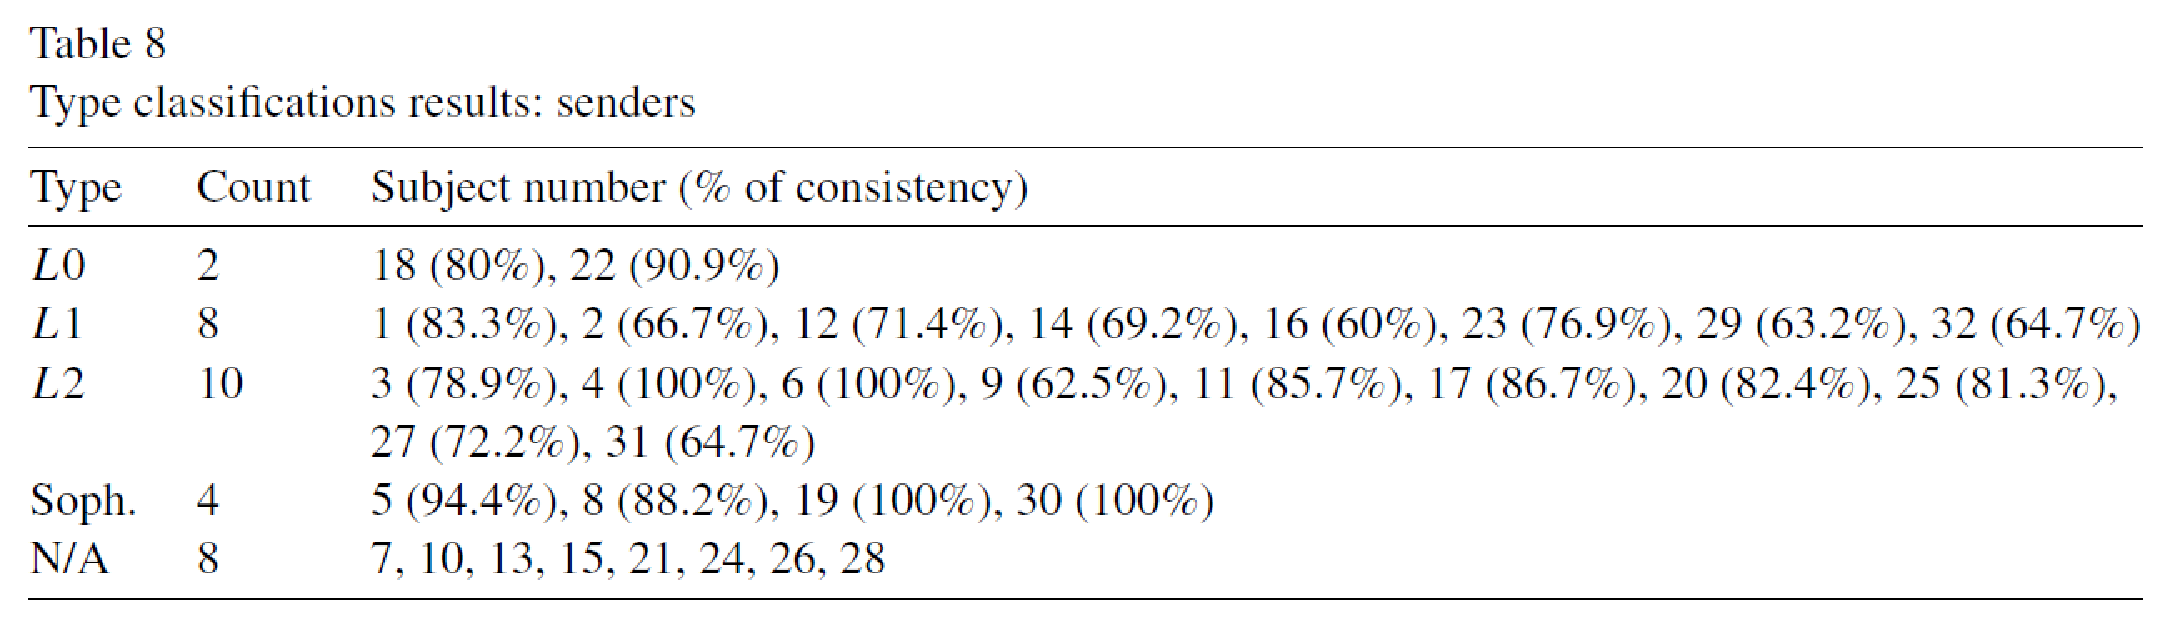
\includegraphics[width=0.98\textwidth]{./i/cw2006Tbl8.eps}\end{center}
\end{card}
\end{frame}
\begin{frame}{Cai \& Wang (GEB 2006)}
\begin{card}
\begin{center}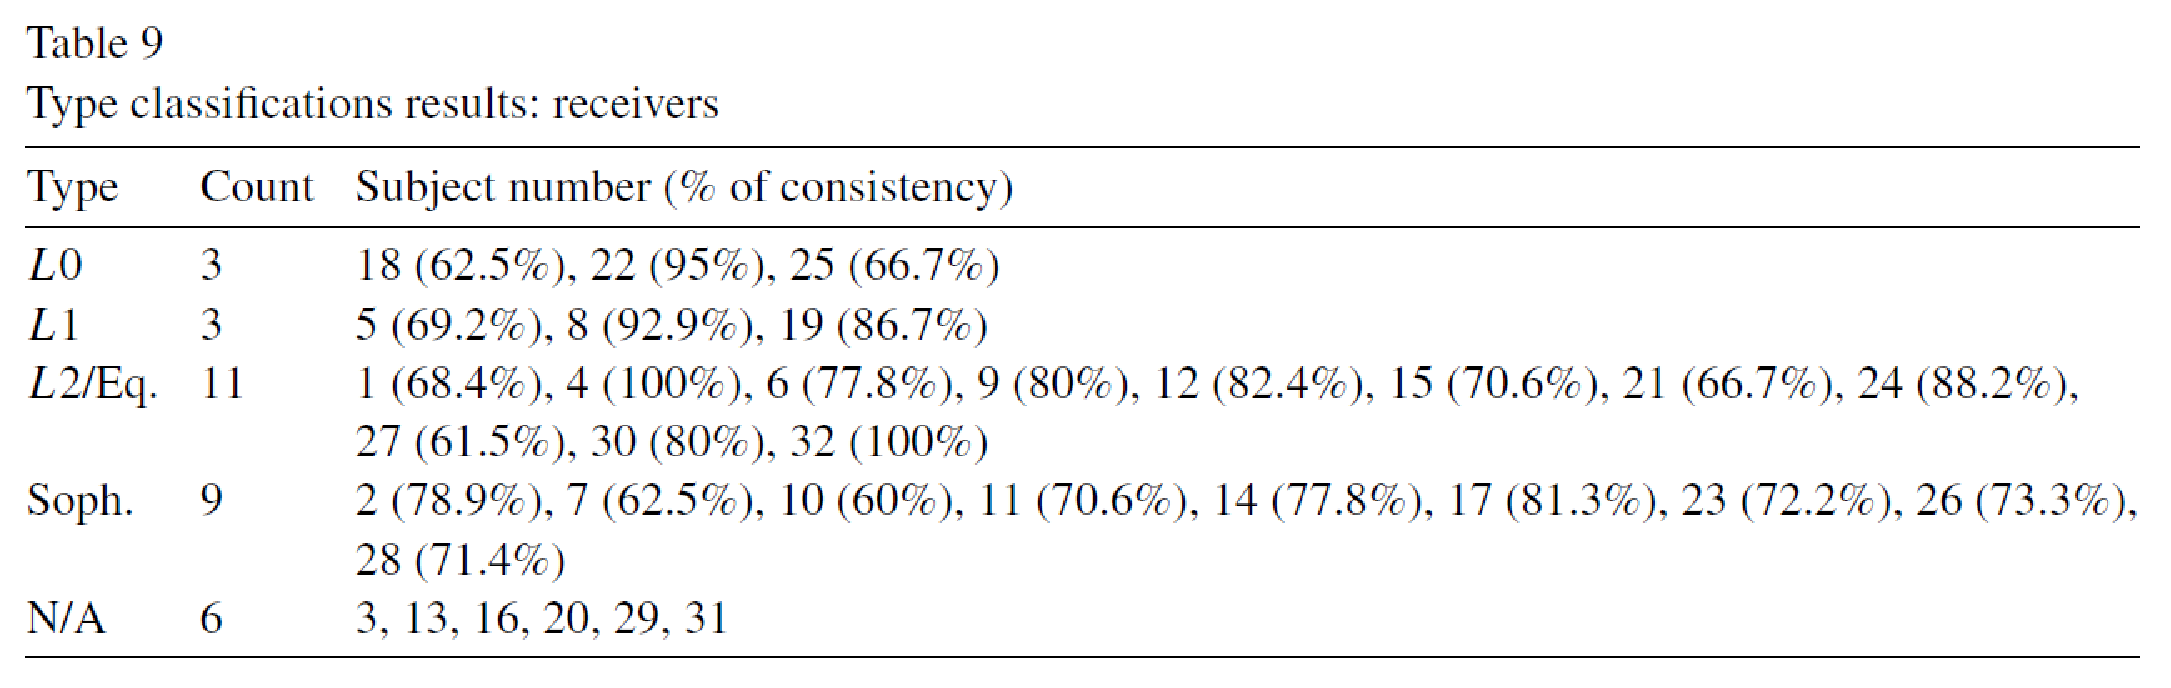
\includegraphics[width=0.98\textwidth]{./i/cw2006Tbl9.eps}\end{center}
\end{card}
\end{frame}
\begin{frame}
\begin{card}[QRE Model: Behavioral Strategies]
			$$p(\theta,m)=\Pr\left\{m\left| \theta\right. \right\}= \frac{\text{exp}\left\{\lambda \hat{u}_\theta(m)\right\}}{\sum_{m^\prime\in M} \text{exp}\left\{\lambda \hat{u}_{\theta}(m^\prime)\right\}}$$
			and
			$$q(m,x)=
			\Pr\left\{x\left| m\right. \right\}= 
			\frac{\text{exp}\left\{\lambda \hat{v}_m(x)\right\} }{\sum_{x^\prime\in X} \text{exp}\left\{\lambda \hat{v}_{m}(x^\prime)\right\}  }$$
\end{card}
\end{frame}

\begin{frame}
    \begin{card}[QRE Model: Expected Payoffs]
    			Sender expected payoff is:
    			$$\hat{u}_\theta(m)=\sum_{x\in X} q(m,x) u(x,\theta)$$
    			
    			Receiver expected payoff is:
    			$$\hat{v}_m(x)=\sum_{\theta\in \Theta} r(\theta\left| m\right. ) v(x,\theta )$$ 
    			
    			where Bayesian posterior tells us:
    			$$r(\theta\left| m\right. )=\frac{p(\theta,m)}{\sum_{\theta^\prime\in\Theta} p(\theta^\prime,m)}$$
    \end{card}
\end{frame}



\begin{frame}
\begin{card}[QRE Model: Equilibrium]
 Need to solve for a fixed point $p^\star$, $q^\star$ where the expected payoff $u^\star$ under the equilibrium strategies lead to exactly those probabilities under the logit-noise model:
 $$p^\star(\theta,m)=\frac{\text{exp}\left\{\lambda \hat{u}^\star_\theta(m;p^\star,q^\star)\right\}}{\sum_{m^\prime\in M} \text{exp}\left\{\lambda \hat{u}^\star_{\theta}(m^\prime;p^\star,q^\star)\right\}}$$
			and
			$$q^\star(m,x)= 
			\frac{\text{exp}\left\{\lambda \hat{v}^\star_m(x;p^\star,q^\star)\right\} }{\sum_{x^\prime\in X} \text{exp}\left\{\lambda \hat{v}^\star_{m}(x^\prime;p^\star,q^\star)\right\}  }$$
\end{card}
\end{frame}

\begin{frame}{Cai \& Wang (GEB 2006)}
\begin{card}
	\begin{center}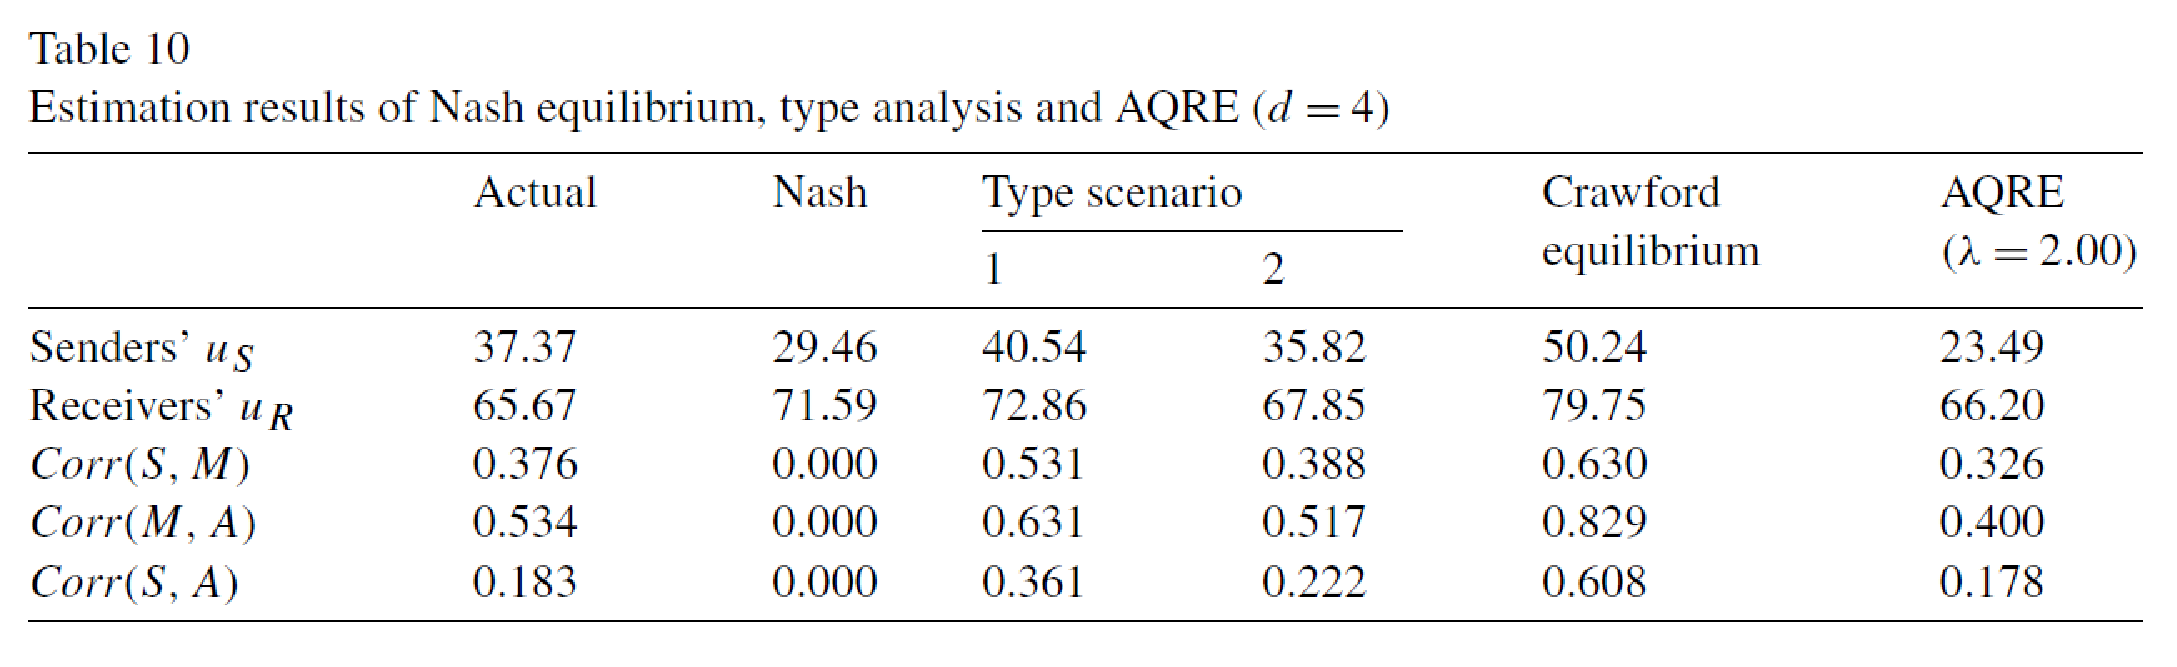
\includegraphics[width=0.98\textwidth]{./i/cw2006Tbl10.eps}\end{center}
\end{card}
\end{frame}

\begin{frame}{Cai \& Wang (GEB 2006)}
\begin{card}
	\begin{itemize}
		\item Main contribution here is in estimating a level-$k$ hierarchy with a focal level-$0$ behavior
		\item Both the QRE and level-$k$ models are explanatory models
		\item Can not pick easily between them
		\item Also, do not know the payoff effects from guilt, other-regarding, etc.
	\end{itemize}
\end{card}
\end{frame}

\section{Gneezy(2005)}
\begin{frame}{Gneezy (2005)}
	\begin{card}
	 Sender finds out the payoffs to the division of a pie:
		\begin{enumerate}[A]
			\item You get \$5, the other player gets \$15
			\item You get \$15, the other player gets \$5
		\end{enumerate}
		Sender then chooses a message from:
		\begin{enumerate}[a]
			\item ``Option A will earn you more money than Option B''
			\item ``Option B will earn you more money than Option A''
		\end{enumerate}
		A receiver gets the message and makes a choice from \emph{A} and \emph{B}
	\end{card}
\end{frame}



\begin{frame}
	\begin{card}[Treatments]
	\centering
		\begin{tabular}{lccc}\toprule
		& & \multicolumn{2}{c}{Payoff to:}\\ \cline{3-4}
		Treatment & Option & Sender & Receiver \\ \midrule
		1		  &   A  & 5 & 6  \\
				  &   B  & 6 & 5  \\
		2		  &   A  & 5 & 15 \\
				  &   B  & 6 & 5  \\
		3		  &   A  & 15 & 5 \\
				  &   B  & 5 & 15 \\ \bottomrule	  
		\end{tabular}
	\end{card}
\end{frame}
\begin{frame}{Gneezy (2005)}
\begin{card}
	\begin{itemize}
		\item Majority of the messages suggestions are followed (approximately 80\%)
		\item Runs a dictator game control where the Sender subject just imposes the outcome choice from the $A$ and $B$
		\item Idea here is to look at preferences over dishonesty through the comparison (differencing out other-regarding concerns)
	\end{itemize}
\end{card}
\end{frame}

\begin{frame}{Gneezy (2005)}
\begin{card}
	\begin{center}
		\begin{tabular}{lccc}\toprule
		& \multicolumn{3}{c}{Selfish Allocation B }\\ \cmidrule{2-4}
		Game & {\small (5,6)v.(6,5)} & {\small (5,15)v.(6,5)} & {\small (5,15)v.(15,5)} \\ \midrule
		Cheap Talk &   $0.36$  & $0.17$ & $0.52$  \\
		Dictator   &   $0.66$  & $0.42$ & $0.90$  \\ \bottomrule	  
		\end{tabular}
	\end{center}
\end{card}	

\begin{card}
    	\begin{itemize}
    		\item Aversion to deceiving others
    		\item 38\% of the subjects would rather be honest than get \$10 extra for themselves
    		\item Statistically significant differences across Game.
    	\end{itemize}
    \end{card}
\end{frame}

\begin{frame}{Gneezy (2005)}
\begin{card}
	\begin{itemize}
		\item Receivers do not know the possible set of states
		\item No theoretical frame through which to understand this
		\item Unclear why Israeli students were paid in dollars, or what currency is here
	\end{itemize}
\end{card}
\end{frame}

\begin{frame}{Fischbacher \& F\"ollmi-Heusi (JEEA 2013)}
\begin{card}
	\begin{itemize}
		\item Similar results to the Gneezy paper, cleaner design
		\item Subjects give a die at their desks
		\item Asked to roll the die and report their result
		\item Payoffs for reports: 
		\begin{itemize}
			\item Six yields nothing; 
			\item One to five yields that many swiss francs
		\end{itemize}
	\end{itemize}
\end{card}
\end{frame}

\begin{frame}{Reports in Baseline}
\begin{card}
	\begin{center}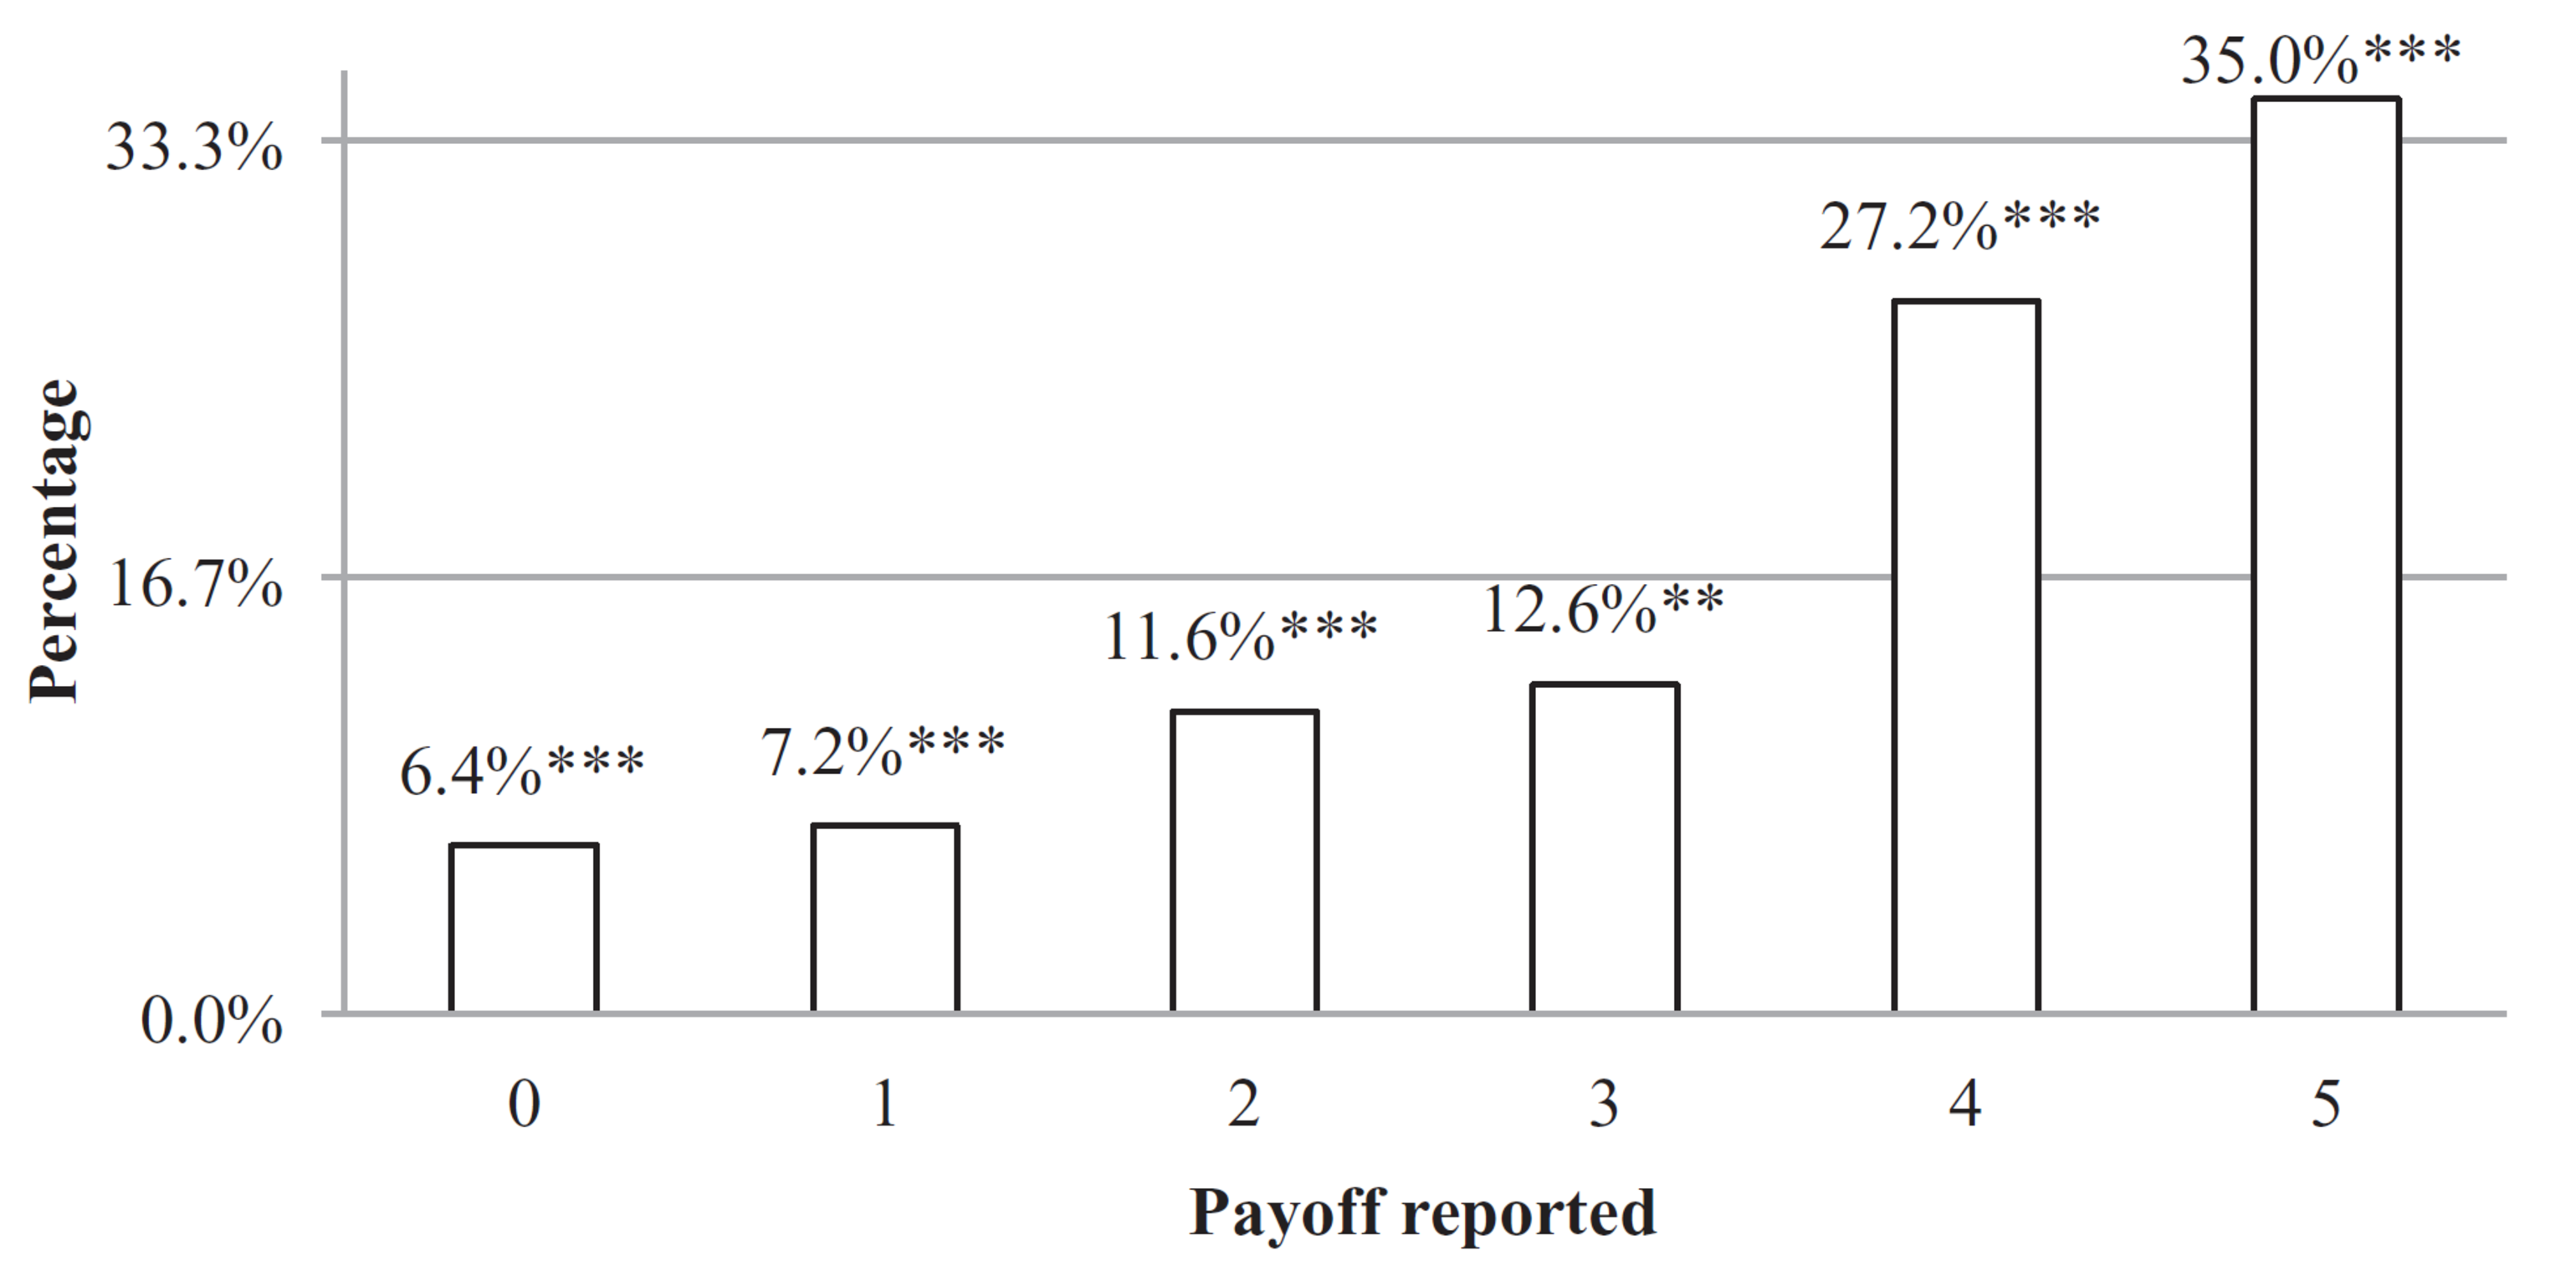
\includegraphics[width=0.96\textwidth]{./i/ffh2013fig1.eps}\end{center}
\end{card}
	
\begin{card}Tests are against a binomial with $p=\frac{1}{6}$\end{card}
\end{frame}

\section{Wang, Spezio \& Camerer (AER 2010))}
\begin{frame}{Wang, Spezio \& Camerer (AER 2010)}
	\begin{card}
		Cai \& Wang (2006) with:
		\begin{itemize}
			\item Eye-tracking
			\item Pupil Dilation
			\item Reaction times
		\end{itemize}
		Preferences are again 
				$$u^R(x,\theta)=C_R-a\cdot \left|x-\theta\right|^{1.4}$$
				and for the sender are:
				$$v^S(x,\theta;d)=C_S-a\cdot \left|x+d-\theta\right|^{1.4}$$
	\end{card}
\end{frame}

\begin{frame}
\begin{card}[Experimental Details:]
	\begin{itemize}
		\item Caltech undergrads
		\item Within-subject design
		\item Two senders were eye-tracked
		\item Six subjects in a session
		\item 45 rounds
		\item Six sessions 
		\item Perturb payoffs to stop memory effects
	\end{itemize}
	\end{card}
\end{frame}

\begin{frame}{Wang, Spezio \& Camerer (AER 2010)}
\begin{card}
    \begin{center}
    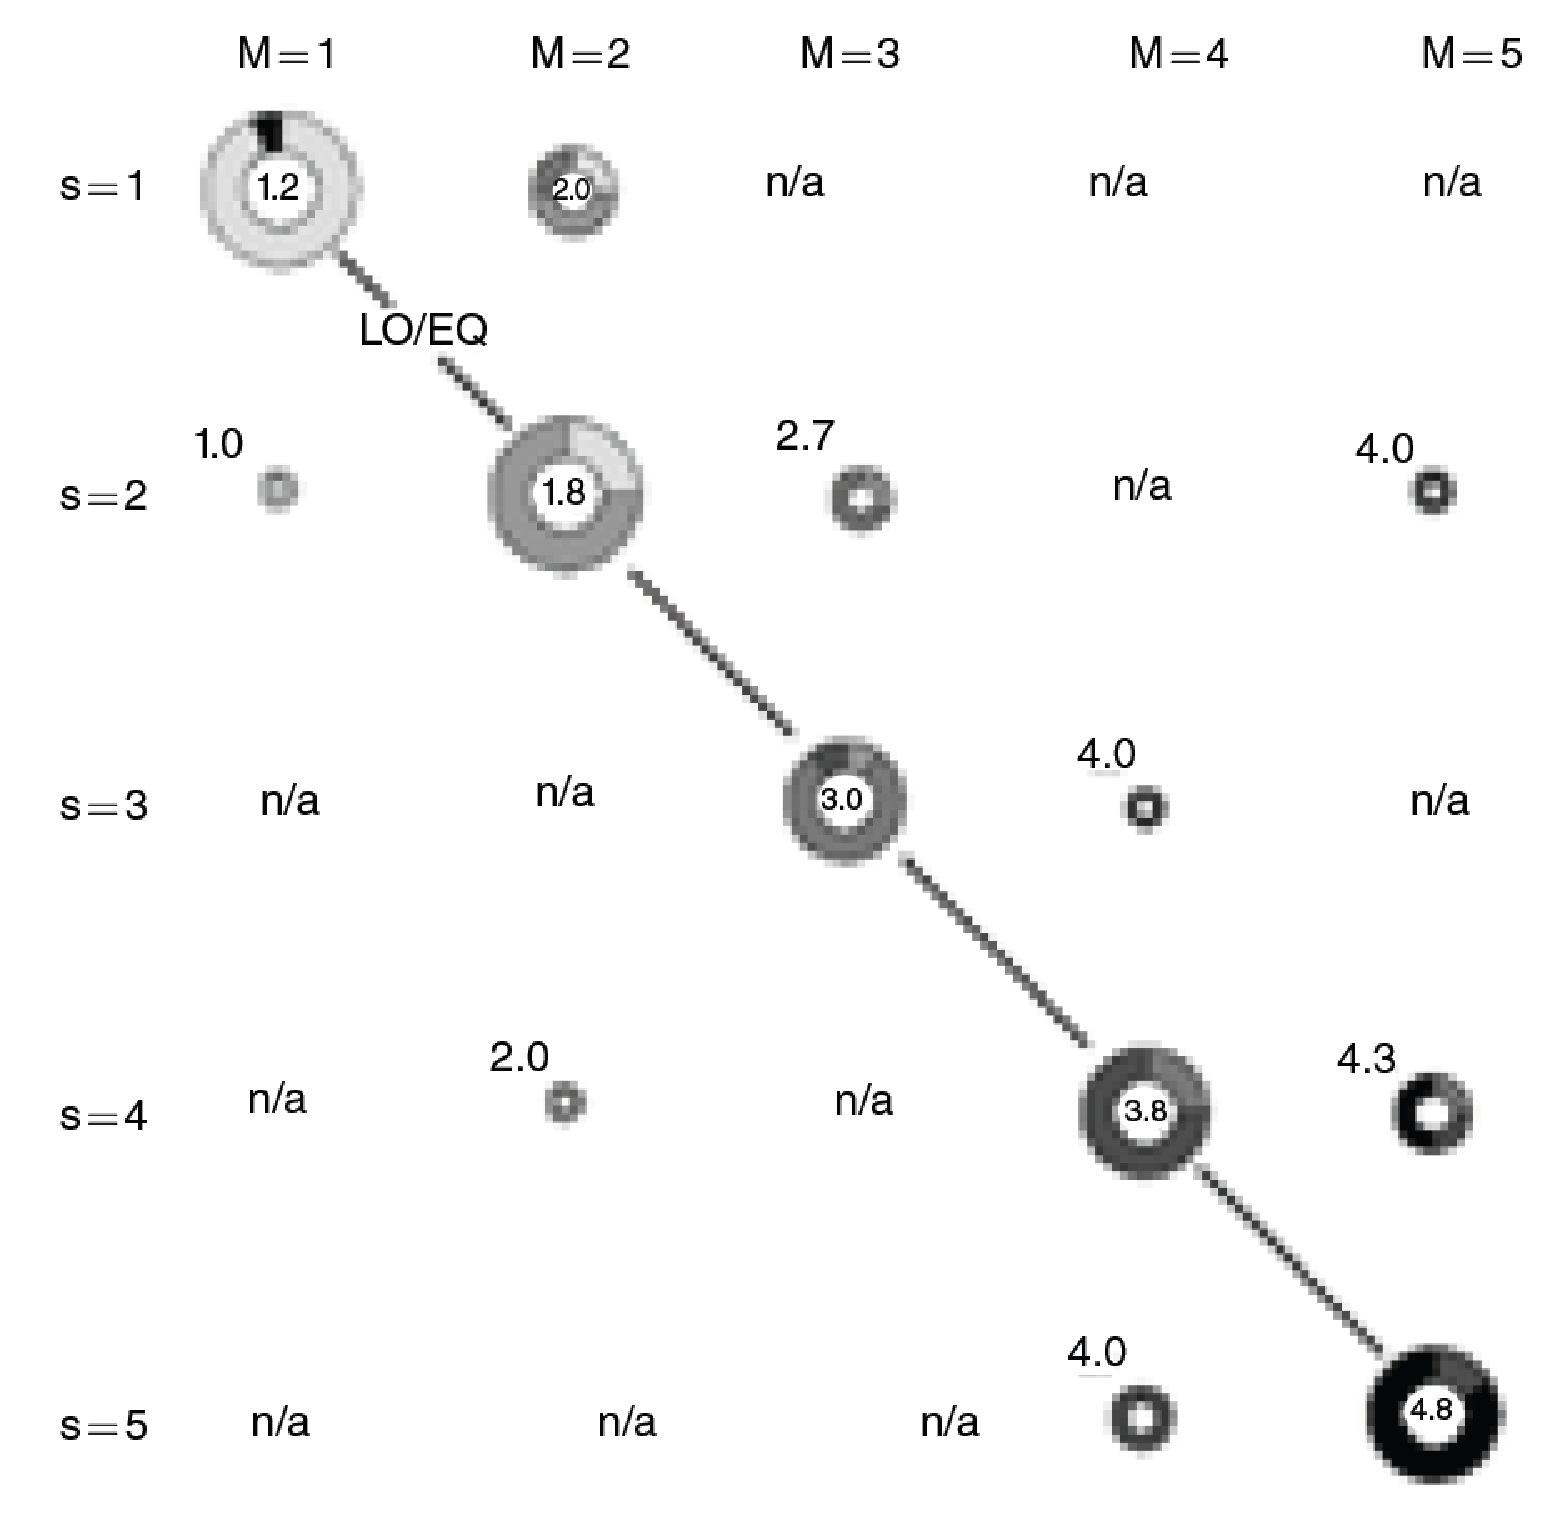
\includegraphics[width=0.6\textwidth]{./i/wsc2010Fig1.eps}
    \end{center}
\end{card}
\end{frame}

\begin{frame}{Wang, Spezio \& Camerer (AER 2010)}
\begin{card}
    \begin{center}
    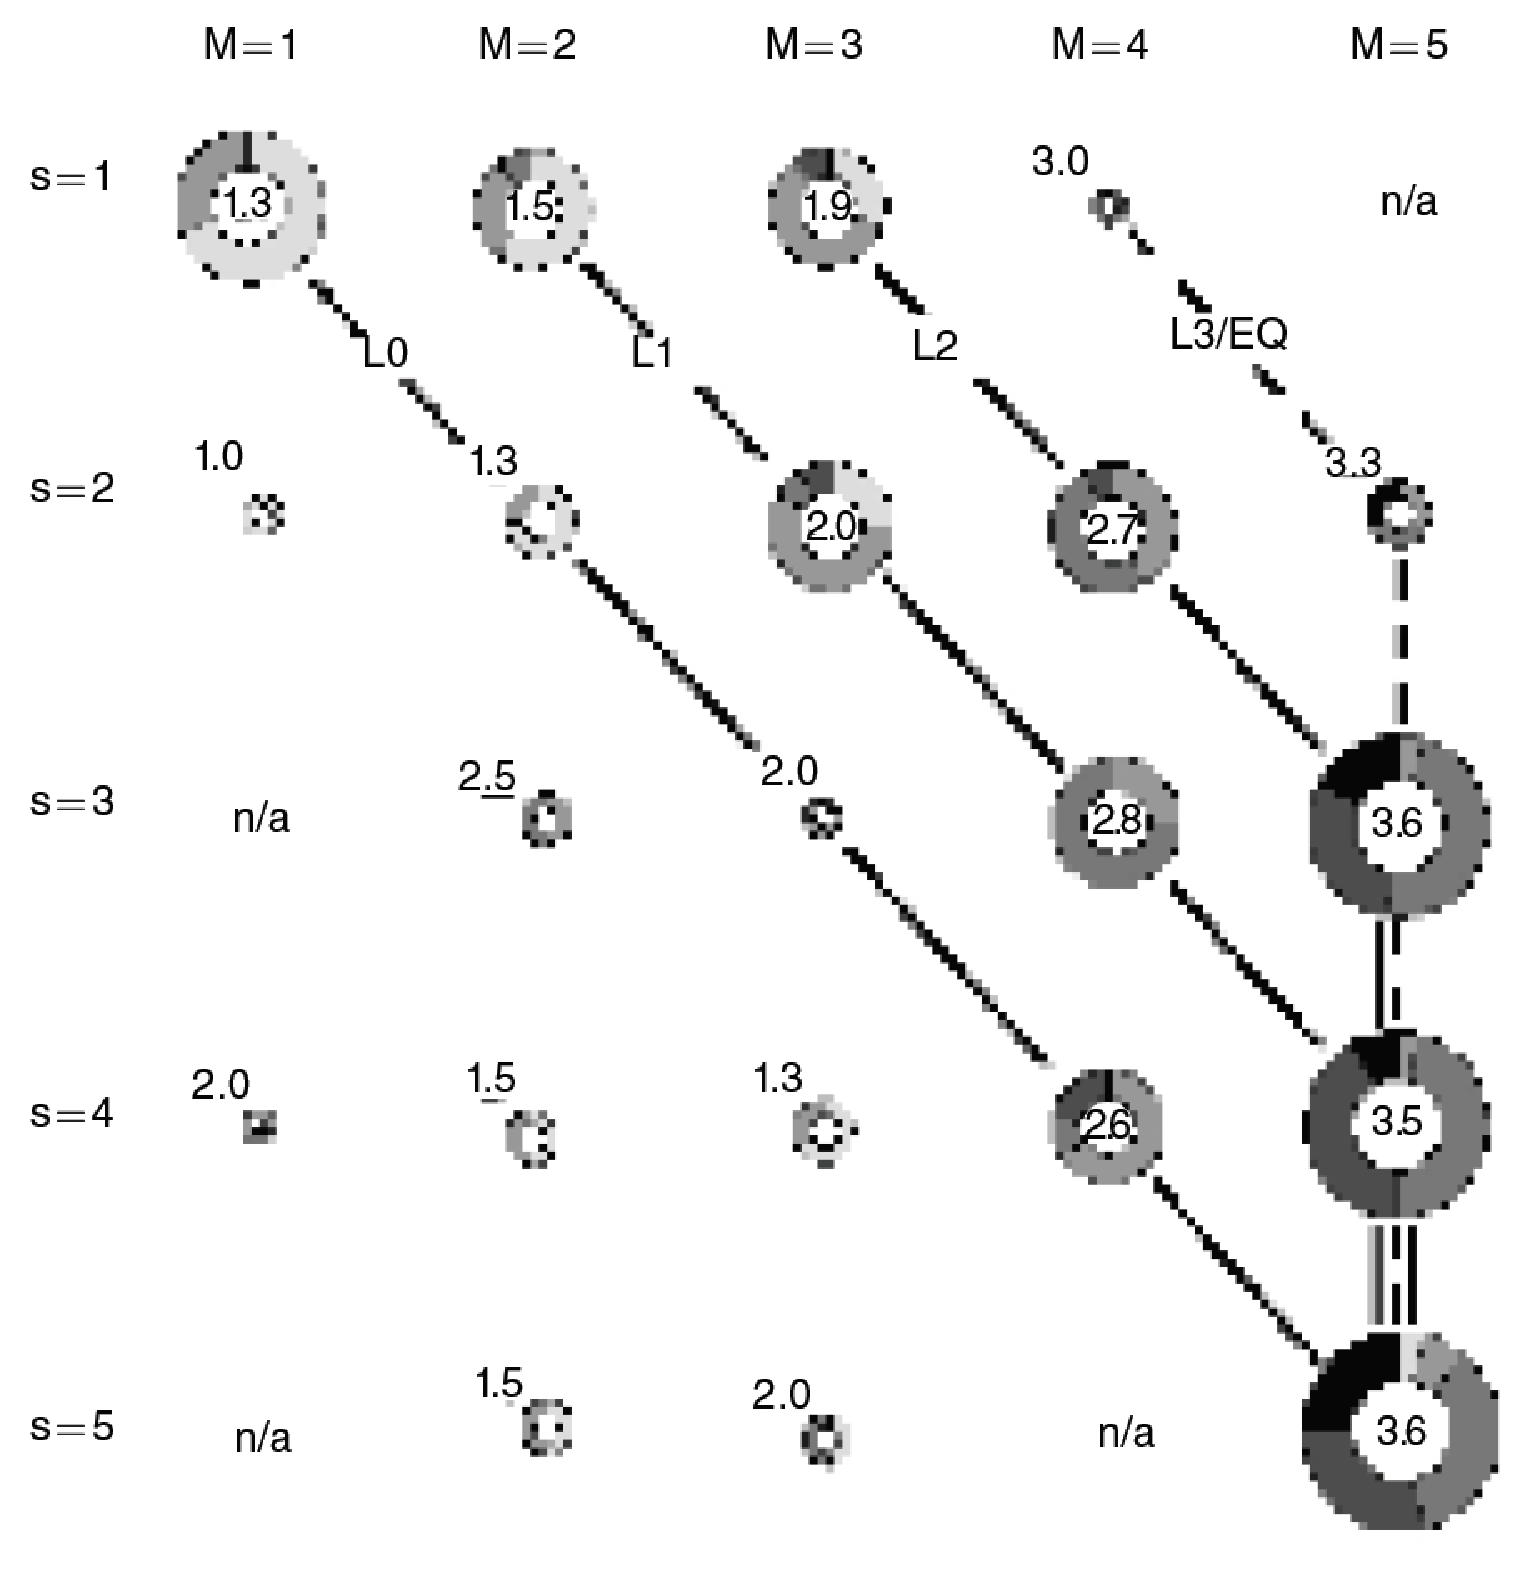
\includegraphics[width=0.6\textwidth]{./i/wsc2010Fig2.eps}
    \end{center}
\end{card}
\end{frame}

\begin{frame}{Wang, Spezio \& Camerer (AER 2010)}
\begin{card}
    \begin{center}
    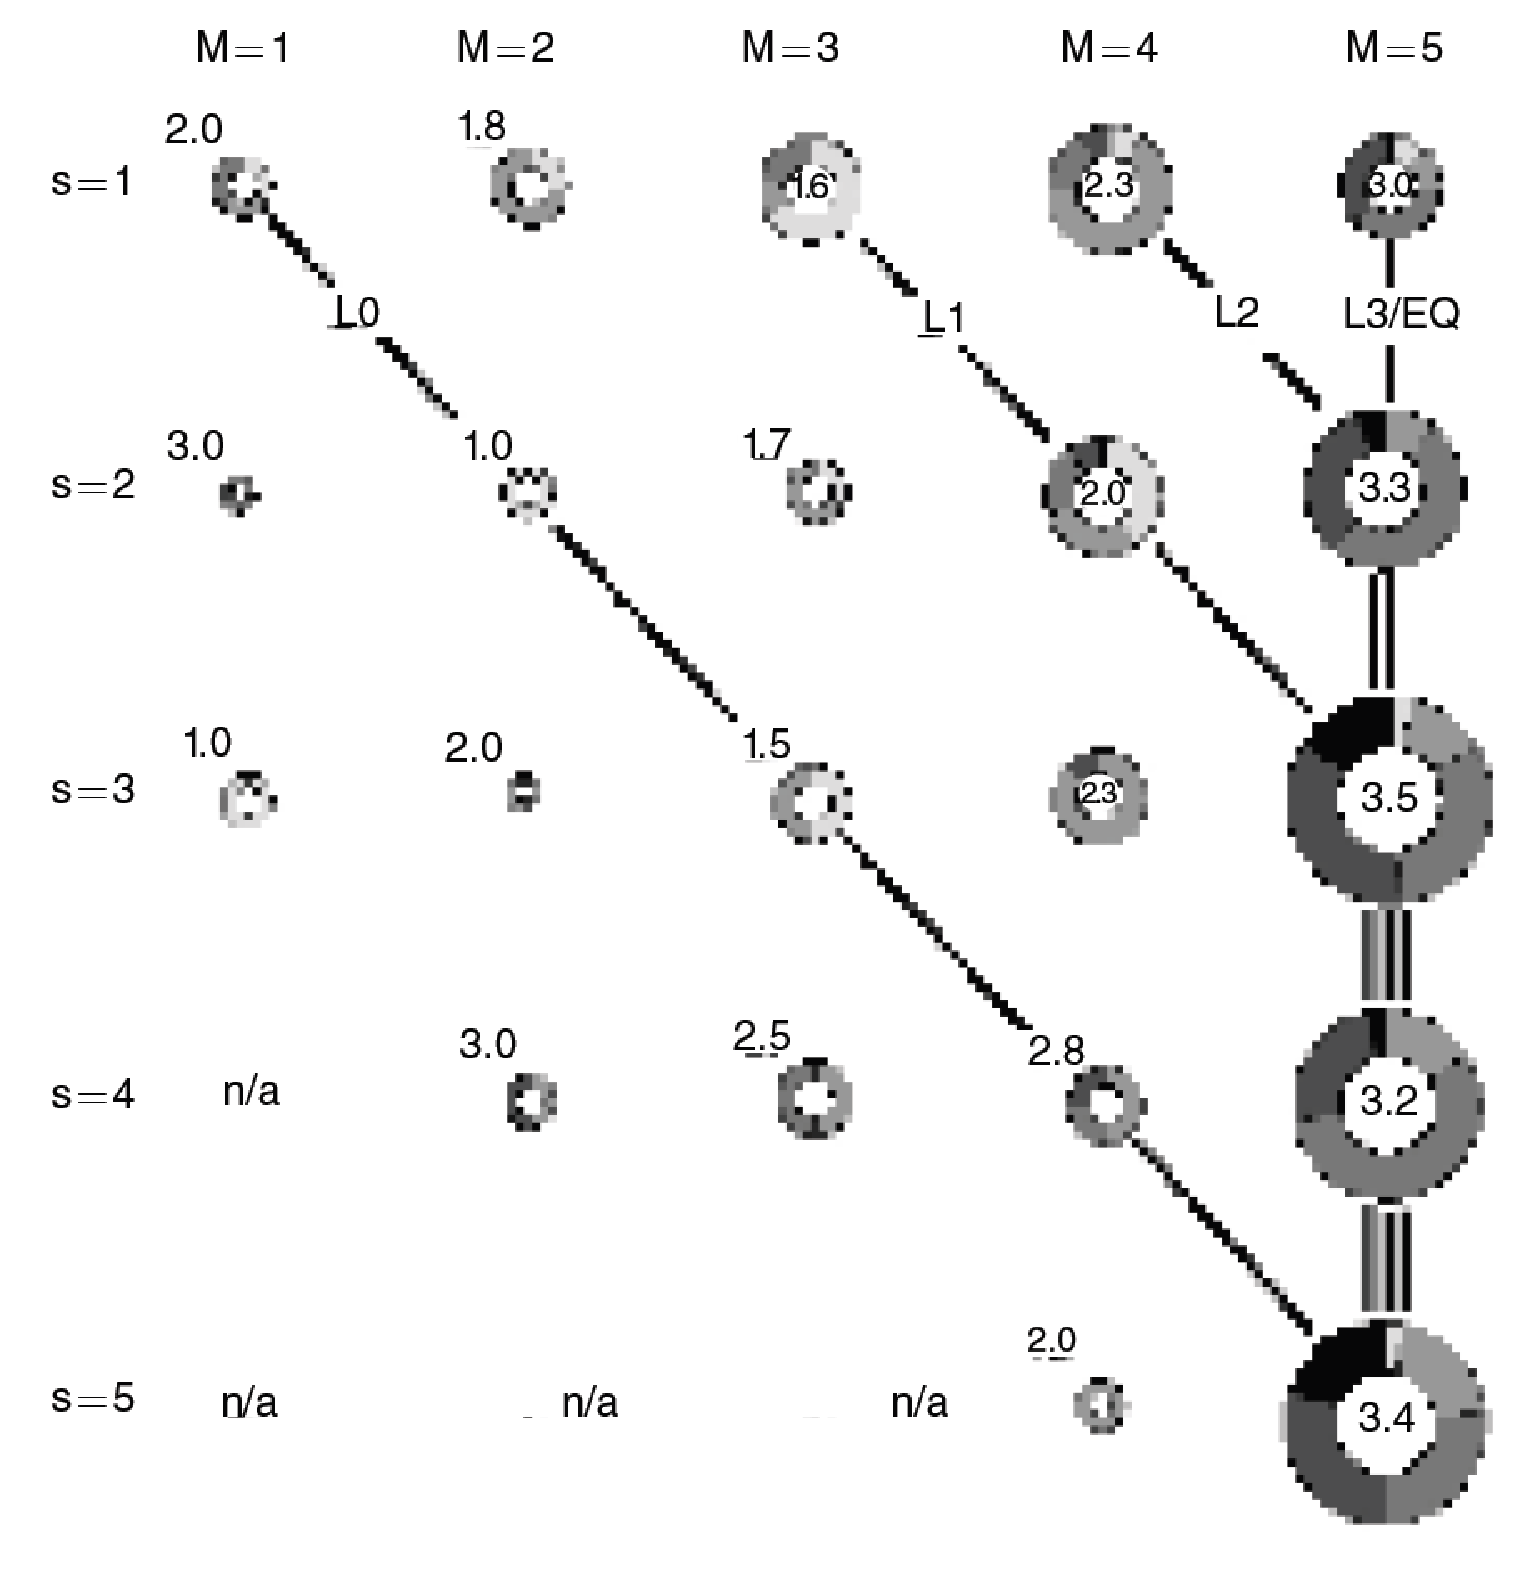
\includegraphics[width=0.6\textwidth]{./i/wsc2010Fig3.eps}
    \end{center}
\end{card}
\end{frame}
\begin{frame}{Wang, Spezio \& Camerer (AER 2010)}
	\begin{card}
Estimate the sender's level types using a spiked-logit model.
		\begin{itemize}
			\item $(1-\epsilon)$ probability of playing level-$k$
			\item $\epsilon$  probability of QRE-type-model around level-$k$ strategy/beliefs with free parameter $\lambda$
		\end{itemize}
		Subject Estimate is a probability of being each level-$k$ type $\mathbf{p}$, $\epsilon$ and $\lambda$
	\end{card}
\end{frame}

\begin{frame}{Wang, Spezio \& Camerer (AER 2010)}
\begin{card}
	\begin{center}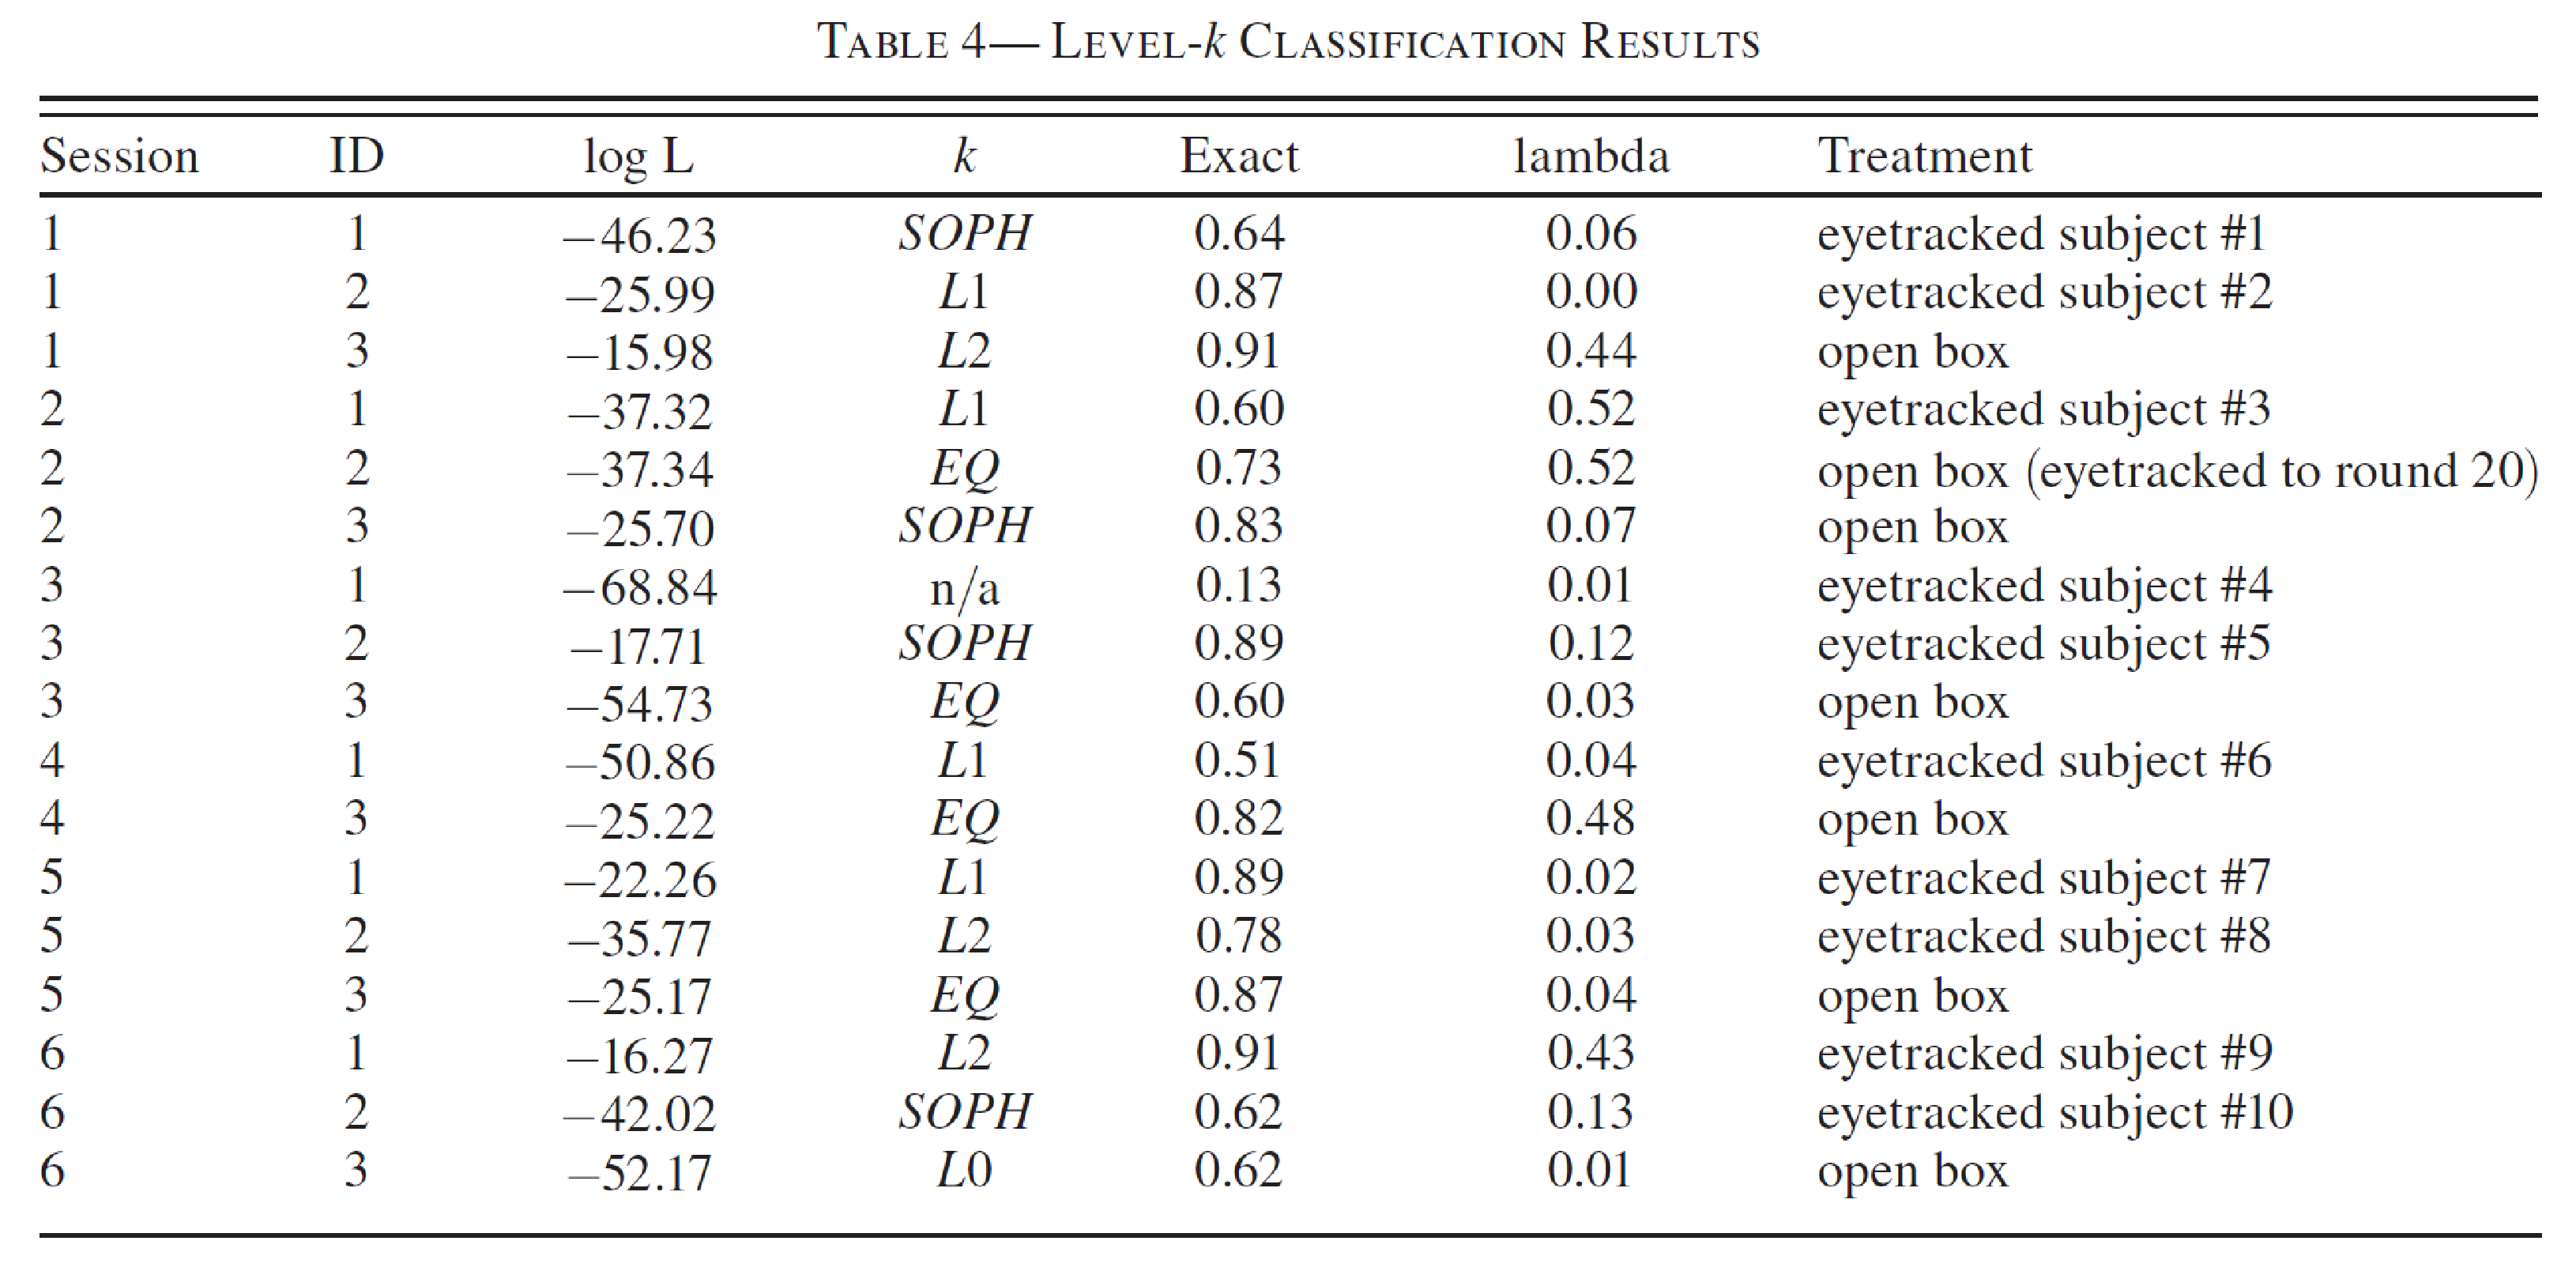
\includegraphics[width=0.98\textwidth]{./i/wsc2010Tbl4.eps}\end{center}
\end{card}
    \begin{card}
    Mostly above 60\% probability on type, with similar mix of behavioral types to Cai \& Wang
    \end{card}
\end{frame}

\begin{frame}{Eye-Lookup Lengths Level 1 $b=1$}
\begin{card}
\includegraphics<1>[width=0.99\textwidth]{./i/wsc2010Fig4.eps}

\end{card}
\end{frame}

\begin{frame}{Eye-Lookup Lengths Level 2 $b=1$}
    \begin{card}
    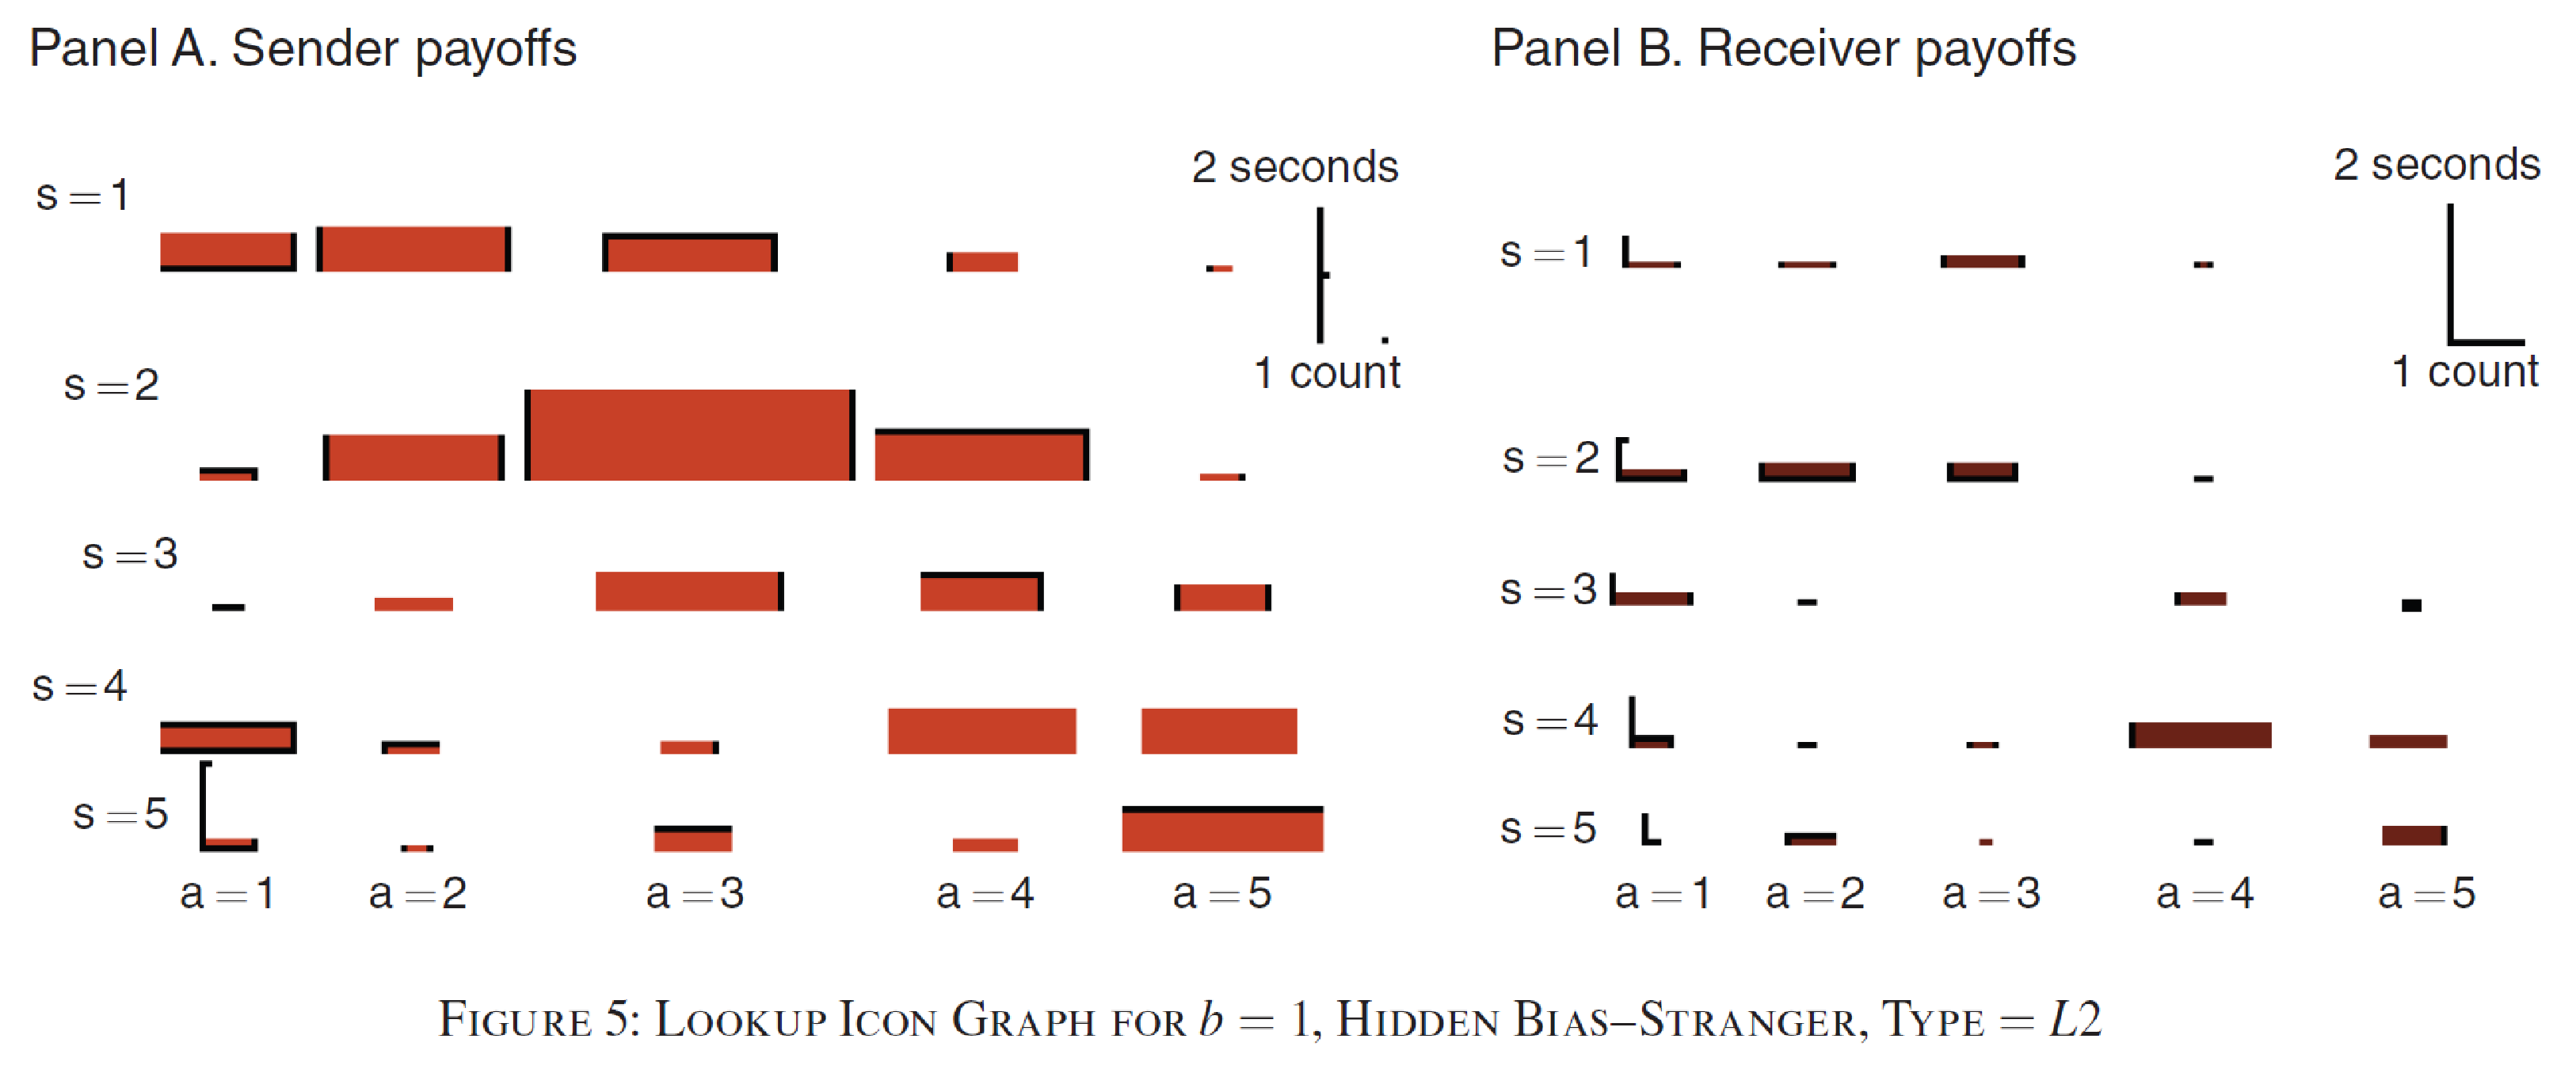
\includegraphics[width=0.99\textwidth]{./i/wsc2010Fig5.eps}
    \end{card}
\end{frame}

\begin{frame}{Eye-Lookup Lengths Level 1 $b=2$}
\begin{card}
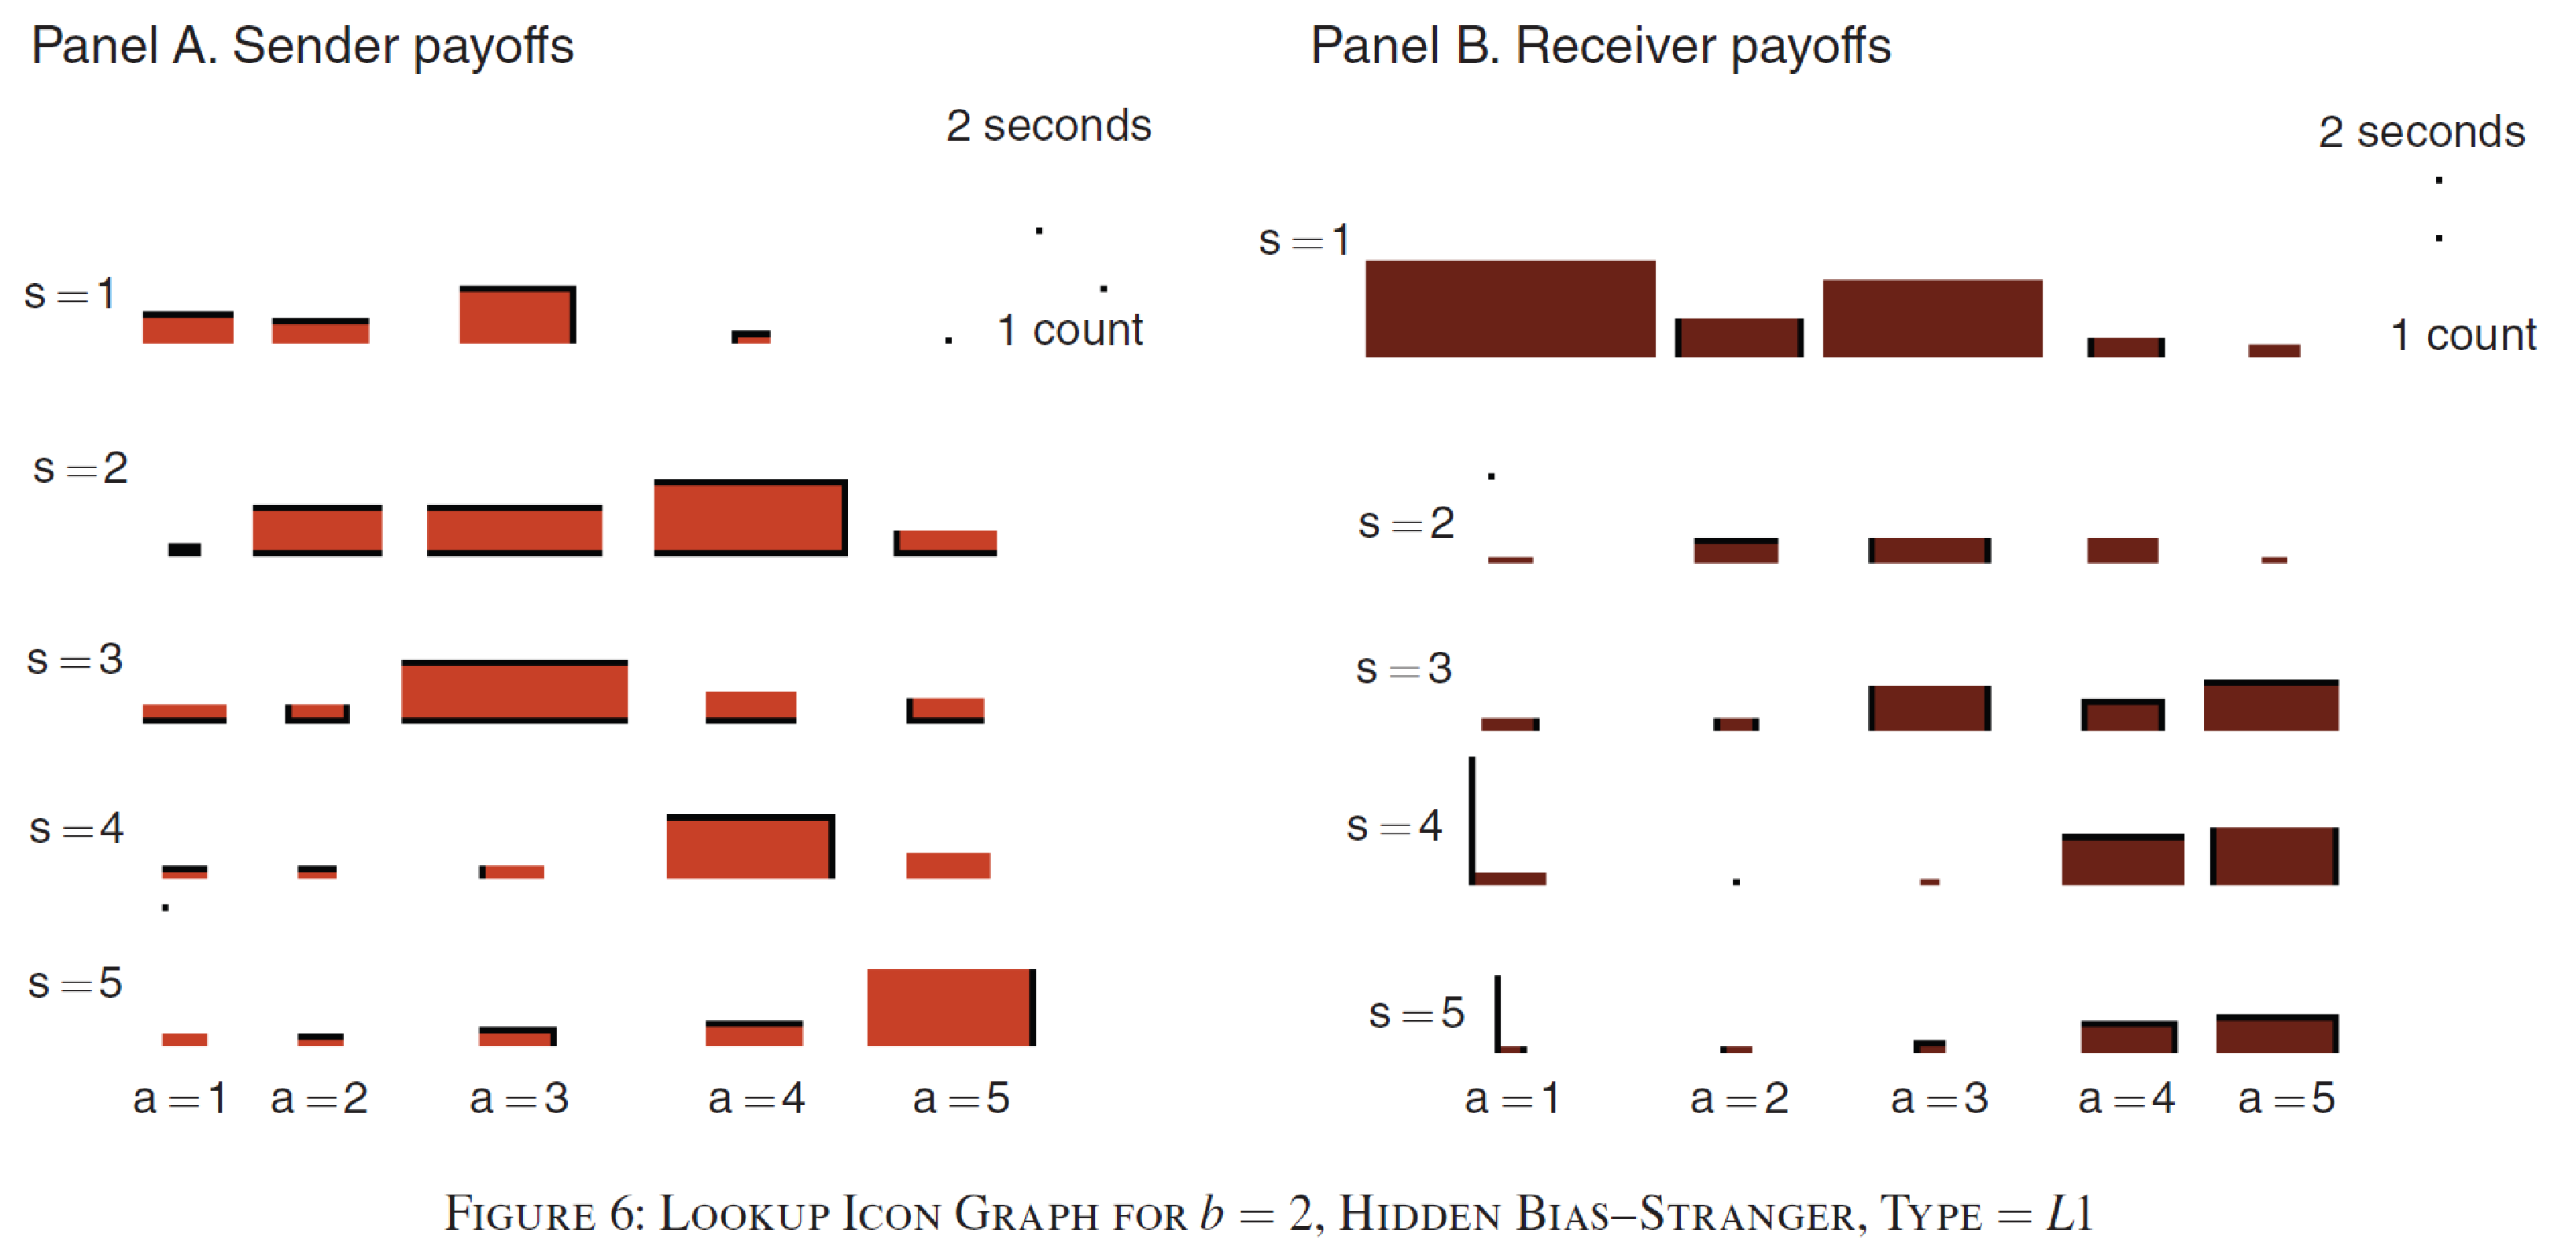
\includegraphics[width=0.99\textwidth]{./i/wsc2010Fig6.eps}
\end{card}
\end{frame}

\begin{frame}{Eye-Lookup Lengths Level 2 $b=2$}
\begin{card}
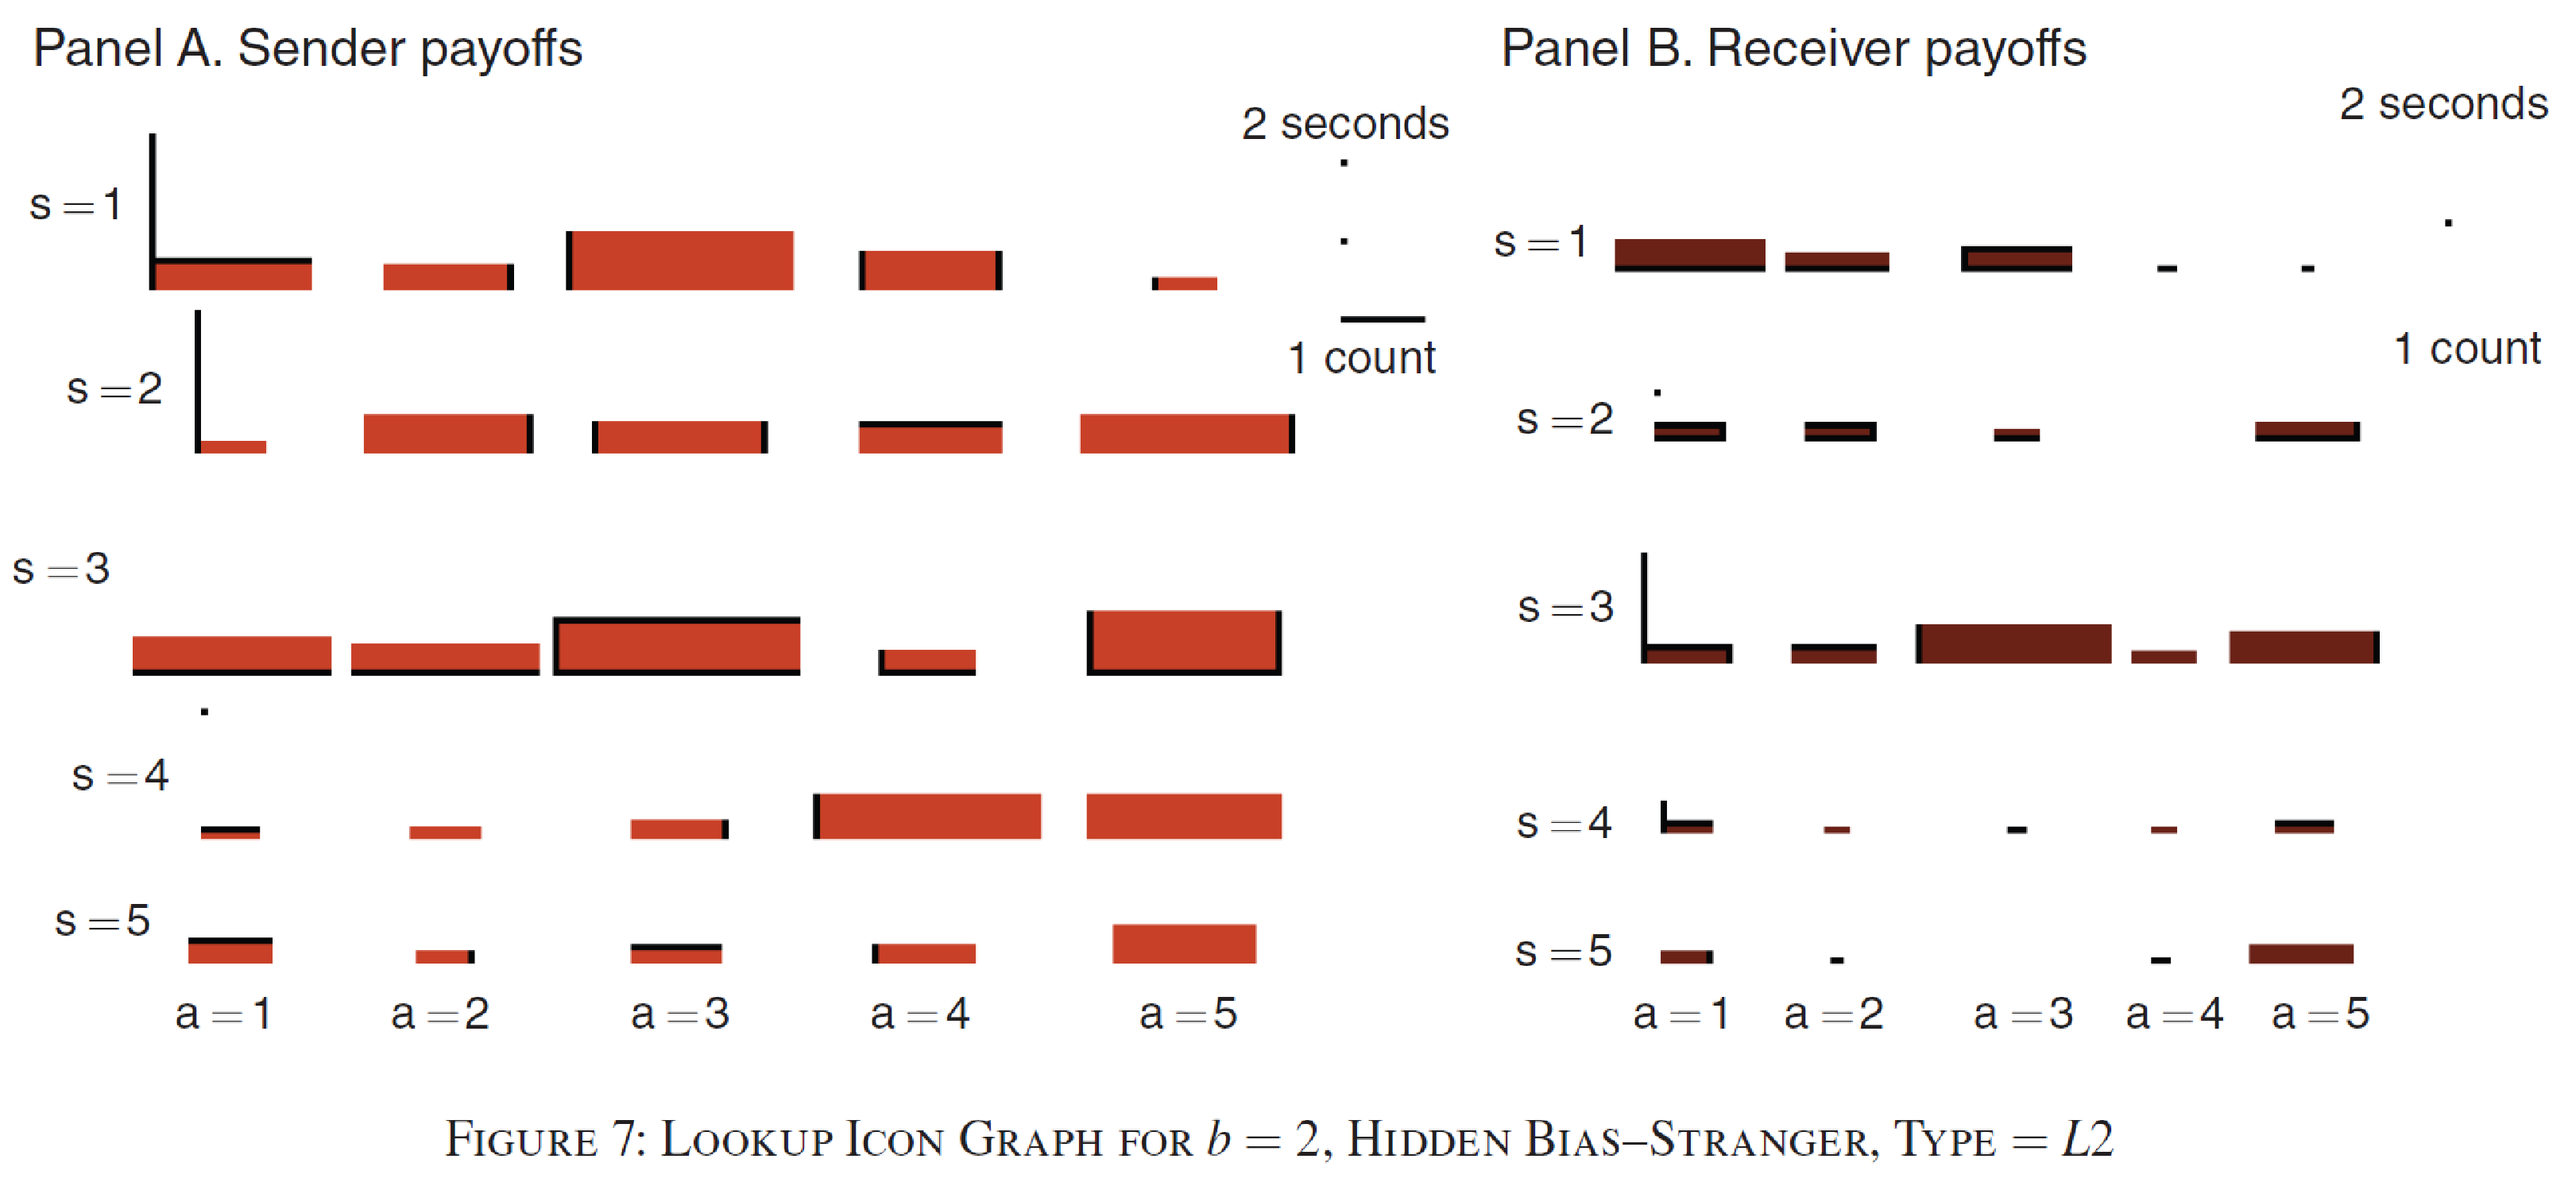
\includegraphics[width=0.99\textwidth]{./i/wsc2010Fig7.eps}
\end{card}
\end{frame}

\begin{frame}{Wang, Spezio \& Camerer (AER 2010)}
\begin{card}
	\begin{itemize}
		\item Subject senders do not spend enough time considering receiver's payoffs
		\item Level-estimations are broadly confirmed in consideration of own payoff lookups
	\end{itemize}
\end{card}
\end{frame}

\begin{frame}{Wang, Spezio \& Camerer (AER 2010)}
    \begin{card}
    	\begin{itemize}
    		\item Pupil dilation and eye-movements can be used to diagnose deceptive messages
    		\item Conclude that their estimated model of behavior can do 20\% better than receivers at figuring out the problem\pause
    		\item Again, no real information on other-regarding concerns
    		\item Not really sure on the economic significance of this part
    		\item Main take-away seems to be further validation of the level-$k$ behavioral model
    	\end{itemize}
    \end{card}
\end{frame}

\end{document}
